\newpage

\begin{appendices}

\section{MIBC Paper images}

\subsection{TCGA}

\begin{figure}[!htb]    
    \centering
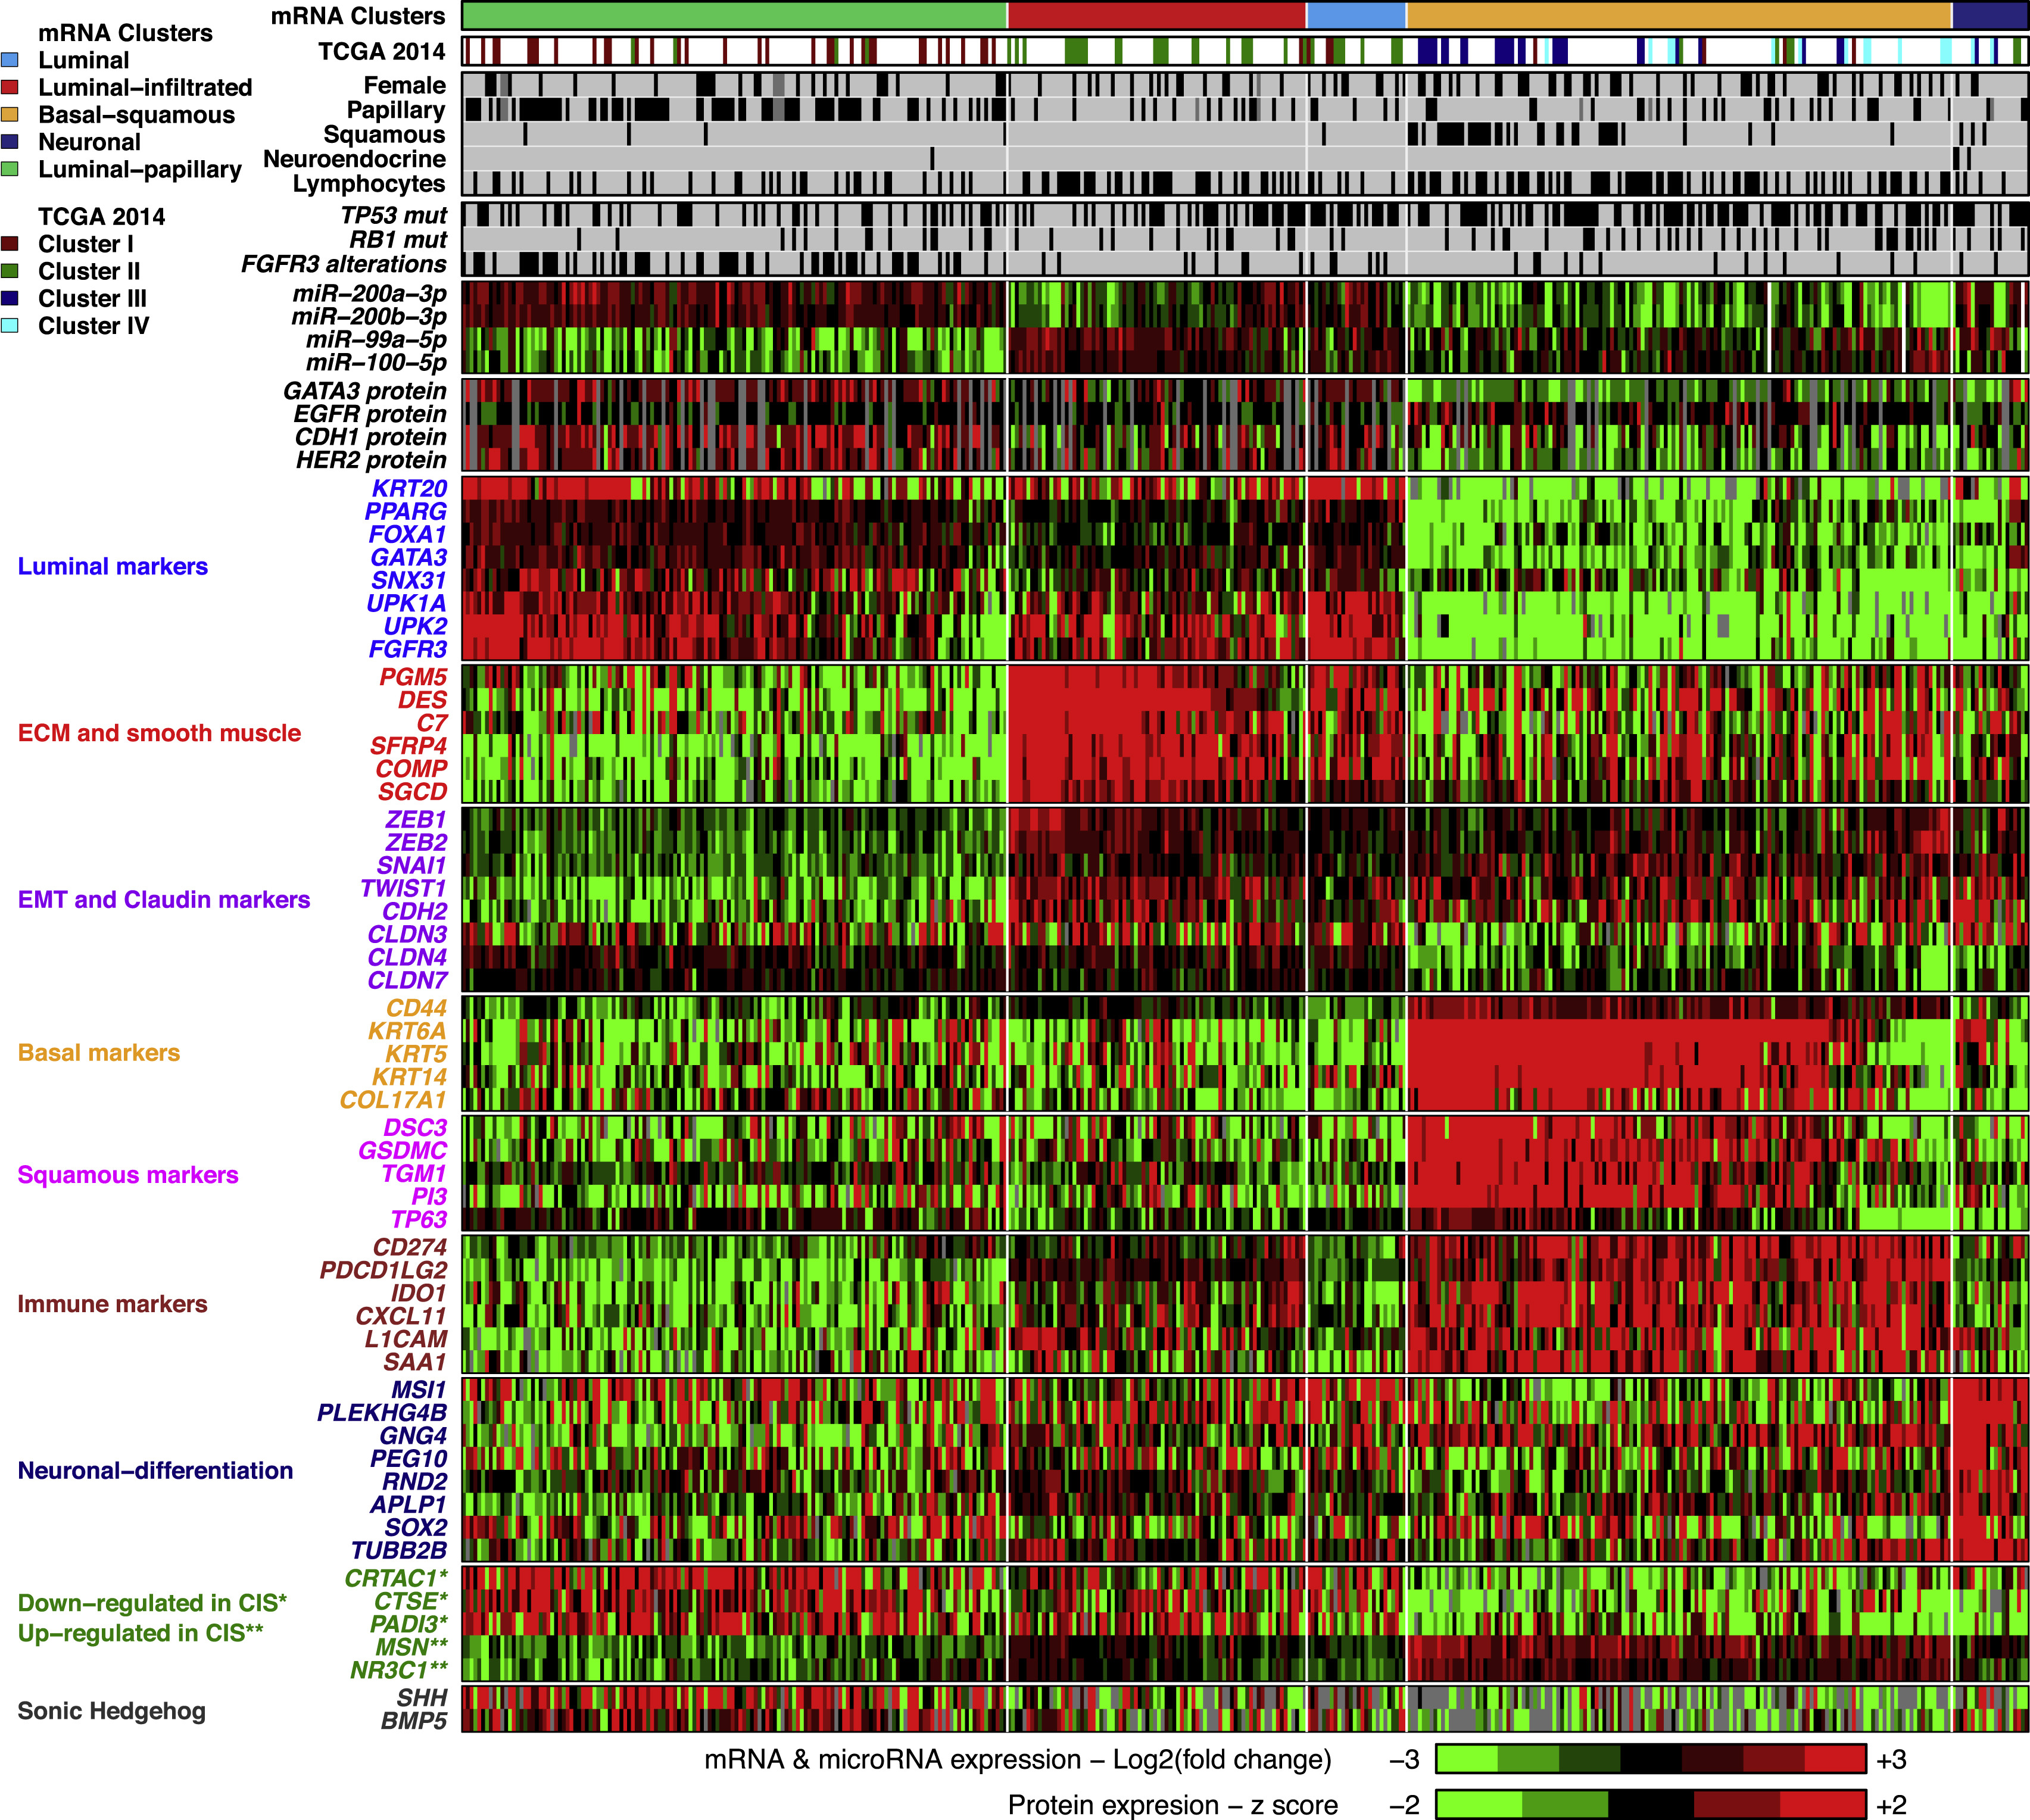
\includegraphics[width=0.9\textwidth,height=0.9\textheight,keepaspectratio]{Sections/Lit_review/Resources/TCGA_2017_subtypes.jpg}
    \caption{Figure 2 from from \cite{Robertson2017-mg} showing the five different molecular subtypes found in the MIBC cohort from TCGA. See \cref{s:lit:tcga_mibc} for a more detailed overviews.}
    \label{fig:ap:tcga_subtypes}
\end{figure}

% MIBC subtypes
\section{MIBC tables subtypes}

\subsection{TCGA}

% TCGA table
\begin{table}[H]
\centering
\caption{The molecular characterisation of the TCGA subgroups taken from the \textit{mRNA Expression-Based Molecular Subtypes} and \textit{Discussion} Figure 2 from \cite{Robertson2017-mg}}
    \begin{tabularx}{\textwidth}{
      >{\hsize=.6\hsize\raggedright\arraybackslash}X
      >{\hsize=.8\hsize\raggedright\arraybackslash}X
      >{\hsize=.6\hsize\arraybackslash}X
    }
    \toprule
    Subtype & Genes & Description \\
    \midrule
    Luminal-papillary (35\%) & \textit{KRT20, PPARG, FOXA1, GATA3, SNX31, UPK1A, UPK2, FGFR3} & 
    \begin{itemize}[leftmargin=*, nosep, after=\vspace{-\baselineskip}, before=\vspace{-.6\baselineskip}]
        \item Characterised by \textit{FGFR3} mutations
        \item Papillary histology
        \item Low risk of progression
    \end{itemize} \\
    \midrule
    Luminal-infiltrated (19\%) & \textit{CD274, PDCD1LG2, IDO1, CXCL11, L1CAM, SAA1} & 
    \begin{itemize}[leftmargin=*, nosep, after=\vspace{-\baselineskip}, before=\vspace{-.6\baselineskip}]
        \item Lowest purity
        \item High expression of \textit{EMT} and myofibroblast markers, and of the miR-200s (tumour suppressor)
        \item Medium expression of \textit{CD274, CTLA4} immune markers
        \item May respond to immune checkpoint therapy
    \end{itemize} \\
    \midrule
    Luminal (6\%) & \textit{KRT20, PPARG, FOXA1, GATA3, SNX31, UPK1A, UPK2, FGFR3} & 
    \begin{itemize}[leftmargin=*, nosep, after=\vspace{-\baselineskip}, before=\vspace{-.6\baselineskip}]
        \item New subtype in TCGA
    \end{itemize} \\
    \midrule
    Basal-squamous (35\%) &\textit{ CD44, KRT6A, KRT5, KRT14, COL17A1}; Squamous: \textit{DSC3, GSDMC, TCGM1, PI3, TP63} & 
    \begin{itemize}[leftmargin=*, nosep, after=\vspace{-\baselineskip}, before=\vspace{-.6\baselineskip}]
        \item High incidence in women
        \item Squamous differentiation, and basal keratin expression
        \item High expression of \textit{CD274, CTLA4} immune markers and may respond immune checkpoint therapy
    \end{itemize} \\
    \midrule
    Neuronal (5\%) &\textit{ MSI1, PLEKHG4B, GNG4, PEG10, RND2, APLP1, SOX2, TUBB2B} & 
    \begin{itemize}[leftmargin=*, nosep, after=\vspace{-\baselineskip}, before=\vspace{-.6\baselineskip}]
        \item Expression of neuroendocrine, neuronal gene and high cell-cycle signature of proliferative state
        \item The most aggressive tumours with the lowest survival rate
    \end{itemize} \\
    \bottomrule
    \end{tabularx}
    \label{tab:lit:tcga_genes}
\end{table}

% Lund
\subsection{Lund}

\begin{table}[H]
\centering
\caption{Summary table of the work done for Lund stratification which is primarily based on the Figure 2 from \citet{Marzouka2018-ge} but it also contains some additional information from research group's earlier work from  \citet{Sjodahl2017-xr}. The suffix '-inf' represents the infiltrated nature of the subtype.}
    \begin{tabularx}{\textwidth}{>{\hsize=.6\hsize\raggedright\arraybackslash}X >{\hsize=\hsize\arraybackslash}X}
    \toprule
    Subtype & Description \\
    \midrule
    UroA and GU & 
    \begin{itemize}[leftmargin=*, nosep, after=\vspace{-\baselineskip}]
        \item The UroA and GU tumours exhibit two signatures known in urothelial cell differentiation 1) \textit{PPARG, FOXA1, GATA3, ELF3} and 2) \textit{UPK1A, UPK1B, UPK2, UPK3A, KRT20}. These are the genes also seen in the Luminal subtypes form TCGA (\textbf{check this}).
        \item The difference between GU and Uro subtypes is given by the up/down-regulated of \textit{FGFR3, CCND1, E2F3, RB1, CDKN2A}.
    \end{itemize} \\
    \midrule
    Basal/Squamous & 
    \begin{itemize}[leftmargin=*, nosep, after=\vspace{-\baselineskip}]
        \item The signatures of \textit{KRT5, KRT14, FOXA1 and GATA3} are definitory for the Basal/Squamous tumours (Ba/Sq). 
        \item Keratinization signature: \textit{KRT5, KRT6A, KRT6B, KRT6C, KRT14, KRT16}
        \item Cell adhesion genes \textit{EPCAM, CDH1, CDH3} differentiate the Basal tumours from the squamous.
        \item The Basal/Squamous are also separated from the Uro and GU subtypes by the difference in expression of the tyrosine kinase receptors \textit{EGFR, ERBB2, ERBB3}.
    \end{itemize} \\
    \midrule
    MES-like & 
    \begin{itemize}[leftmargin=*, nosep, after=\vspace{-\baselineskip}]
        \item Similar to Sc/NE-like, but are less infiltrated
    \end{itemize} \\
    \midrule
    Sc/NE-like & 
    \begin{itemize}[leftmargin=*, nosep, after=\vspace{-\baselineskip}]
        \item As in the case for Basal, high in \textit{KRT5, KRT14}, low in \textit{FOXA1, GATA3}
        \item High expression in\textit{ CHGA, SYP, ENO2}
        \item More infiltrated than the MES-like
    \end{itemize} \\
    \bottomrule
    \end{tabularx}
    \label{tab:lit:lund_genes}
\end{table}



% Consensus
\subsection{Consensus}


\begin{table}[!htb]
\centering
\caption{The molecular characterisation of the MIBC subgroups taken based on the consensus work of \cite{Kamoun2020-tj}. It summaries sections\  textit{3.2 and 3.3} from the main paper. LumP, LumNS and LumU exhibit more differentiation status characteristics and contain \textit{PARG/GATA3/FOXA1}-related Lund signature.}
    \begin{tabularx}{\textwidth}{>{\hsize=.8\hsize\raggedright\arraybackslash}X >{\hsize=\hsize\arraybackslash}X}
    \toprule
    Subtype & Description \\
    \midrule
    Luminal-papillary (LumP) (24\%) & 
    \begin{itemize}[leftmargin=*, nosep, after=\vspace{-\baselineskip}]
        \item High expression of noninvasive Ta pathway signature
        \item Mutations in \textit{FGFR3, KDM6A}
    \end{itemize} \\
    \midrule
    Luminal non-specified (LumNS) (8\%) & 
    \begin{itemize}[leftmargin=*, nosep, after=\vspace{-\baselineskip}]
        \item Elevated stromal infiltration signatures
        \item \textit{ELF3} mutations, activated by \textit{PPARG//RARG}
    \end{itemize} \\
    \midrule
    Luminal unstable (LumU) (15\%) & 
    \begin{itemize}[leftmargin=*, nosep, after=\vspace{-\baselineskip}]
        \item Higher cell activity compared to other luminal tumours
        \item Mutations in \textit{ERCC2, TP53}
    \end{itemize} \\
    \midrule
    Stroma-rich (15\%) & 
    \begin{itemize}[leftmargin=*, nosep, after=\vspace{-\baselineskip}]
        \item Intermediate levels of urothelial differentiation and stromal infiltration
        \item Overexpression of smooth muscle, endothelial, fibroblast and myofibroblast gene signatures
        \item Immune infiltration of T and B-cell
    \end{itemize} \\
    \midrule
    Basal/Squamous (35\%) & 
    \begin{itemize}[leftmargin=*, nosep, after=\vspace{-\baselineskip}]
        \item Mutations in \textit{KDM6A, RB1}
        \item Signatures associated with Basal
        \item Immune infiltration: cytotoxic lymphocytes, natural killer cells
    \end{itemize} \\
    \midrule
    Neuronal (3\%) & 
    \begin{itemize}[leftmargin=*, nosep, after=\vspace{-\baselineskip}]
        \item Mutations in \textit{KDM6A, RB1}
        \item Signatures associated with Basal
    \end{itemize} \\
    \bottomrule
    \end{tabularx}
    \label{tab:lit:consensus_genes}
\end{table}

\newpage


% List of models

\section{List of Models} \label{ap:tables_models}

\newpage

\begin{center}
\begin{small} % Consider switching to \footnotesize or \scriptsize if necessary
\begin{longtable}{|p{3cm}|c|p{1.2cm}|c|p{2.0cm}|p{4.0cm}|}
    \hline \textbf{Model} 
    & \multicolumn{1}{p{1.0cm}|}{\textbf{RNA-seq}} 
    & \multicolumn{1}{p{1.2cm}|}{\textbf{Micro-arrays}} 
    & \multicolumn{1}{p{1.0cm}|}{\textbf{Muta-tions}} 
    & \textbf{Other}
    & \textbf{Approach}  \\ \hline  \hline
    \endfirsthead
    
    \endlastfoot    
    \citet{Cava2018-rv} & x &  &  & Pathways & Network/Graph \\ \hline
    GANPA &  & x &  & Protein-protein & Network/Graph \\ \hline
    LEGO & x &  &  & Pathways & Network/Graph \\ \hline
    Dendrix &  &  & x &  & Greedy algorithm \& Monte Carlo (MCMC) \\ \hline
    MDPFinder & x &  & x &  & EA \& optimisation algorithms \\ \hline
    Neuro-evolution &  & x &  &  & FS-NEAT, feature selection via neuroevolution / supervised \\ \hline
    PICNIC  &  &  & x &  & Pipeline, 4 stages with a range of models \\ \hline
    DriverNet & x &  & x &  & Network/graph \\ \hline
    DawnRank & x &  & x & Gene network & Network/graph. Built on DriverNet \& using PageRank. \\ \hline
    Memo & x &  & x &  & Network/Graphs, Stats \\ \hline
    iPAC & x &  & x &  & Stats \& correlations \\ \hline
    Comet  & x &  & x &  & Submatrix, Markov Chain Monte Carlo  \\ \hline
    \citet{Feltes2019-bd} & x & x &  &  & Built on Neuroevolution \\ \hline
    \citet{Palazzo2019-hx} &  &  & x &  & Autoencoders, hierarchical clustering \\ \hline
    \citet{Chaudhary2018-qj} & x &  &  & miRNA, DNA methylation & Autoencoders \\ \hline
    \citet{Ma2019-hk} & x &  &  & miRNA, DNA methylation & Autoencoders \\ \hline
    TCGA clustering & x &  &  &  & Hierarchical clustering \\ \hline
    Consensus clustering & x &  &  &  & Hierarchical clustering \\ \hline
    \citet{Capecci2020-uj} &  & x & x &  & SNN and EA \\ \hline
    MutsigCV &  &  & x &  & Stats \\ \hline
    \caption{Computational models explored in this literature review with the type of data used and the approaches.}
    \label{tab:data_used}
\end{longtable}
\end{small}
\end{center}
    

    
{\footnotesize % Reduces the font size around the table
\begin{longtable}{|p{3cm}|p{1.8cm}|p{2.2cm}|p{2.8cm}|p{3.5cm}|}
\hline 
\textbf{Model} & \textbf{Data used} & \textbf{Datasets} & \textbf{Approach} & \textbf{Goal} \\ 
\hline 
\endfirsthead

\endlastfoot    
\citet{Cava2018-rv} & Mut & KEGG [5]; TCGA  & Network/Graph & Establish a connection between GE and functional pathways  \\ \hline
GANPA & GE  & GSEA; for PPI -HPRD, MINT, DIP, MINT, IntAct & Network/Graph & Breast cancer, asthma, p53 \\ \hline
LEGO & GE + pathways & KEGG \& others & Network/Graph & Autism and breast cancer \\ \hline
Dendrix & GE & TCGA, Thomas et al. & Greedy algorithm, Monte Carlo & Pan-cancer analysis \\ \hline
MDPFinder & GE + Mut & TCGA & EA, optimisation algorithm & Head \& Neck, glioblastoma and ovarian cancer \\ \hline
Neuro-evolution & GE & GEO & FS-NEAT, feature selection via neuroevolution / supervised & Leukaemia, breast, and colorectal cancers \\ \hline
PICNIC  & Mut & TCGA  & Pipeline, 4 stages with a range of models & Multiple cancer types  \\ \hline
DriverNet & GE + Mut & TCGA, METABRIC, TN and GBM & Network/graph &  Glioblastoma, breast, triple-negative breast, serous ovarian \\ \hline
DawnRank & GE + Mut & TCGA & Network/graph. Built on DriverNet, using PageRank & Breast, ovarian cancer \\ \hline
Memo & GE + Mut & TCGA & Network/ Graphs, Stats & Glioblastoma multiforme (GBM) and ovarian cancer \\ \hline
iPAC & GE + Mut & Multiple datasets & Stats, correlations & Breast \\ \hline
Comet  & GE + Mut & TCGA & Submatrix, Markov Chain Monte Carlo & breast \& gastric cancer, glioblastoma, myeloid leukaemia \\ \hline
\citet{Feltes2019-bd} & GE  & GEO / (Various datasets) & Built on Neuroevolution & Pan-cancer \\ \hline
\citet{Palazzo2019-hx} & Mut & ICGC & Autoencoders, hierarchical clustering & Tumor mutation profile analysis \\ \hline
\citet{Chaudhary2018-qj} & GE + others & TCGA & Autoencoders & Patient survival on liver cancer \\ \hline
\citet{Ma2019-hk} & GE & TCGA, STRING & Autoencoders &  Bladder and Brain Lower Grade Glioma \\ \hline
TCGA clustering & GE & TCGA & Hierarchical clustering & Bladder cancer  \\ \hline
Consensus clustering & GE & TCGA & Hierarchical clustering & Bladder cancer \\ \hline
\citet{Capecci2020-uj} & GE + Mut & TCGA & SNN and EA & Skin dermatitis  \\ \hline
\caption{Datasets: Kyoto Encyclopedia of Genes and Genomes (KEGG) \cite{Kanehisa2017-wj}, The Cancer Genome Atlas (TCGA) \cite{Tcga2018-sj}, \citet{Thomas2007-yj} - "High-throughput oncogene mutation profiling in human cancer", The Gene Expression Omnibus (GEO) \cite{Clough2016-zc, Davis2007-at}, International Cancer Genome Consortium (ICGC) \cite{International_Cancer_Genome_Consortium2010-ca}, Search Tool for Retrieval of Interacting Genes/Proteins(STRING) \cite{Szklarczyk2019-pu}.}
\label{tab:approaches}
\end{longtable}
}

% % Dendogram example
% \section{Dendrogram} \label{ap:dendogram}


% \begin{figure}[!htb]                                  
%     \centering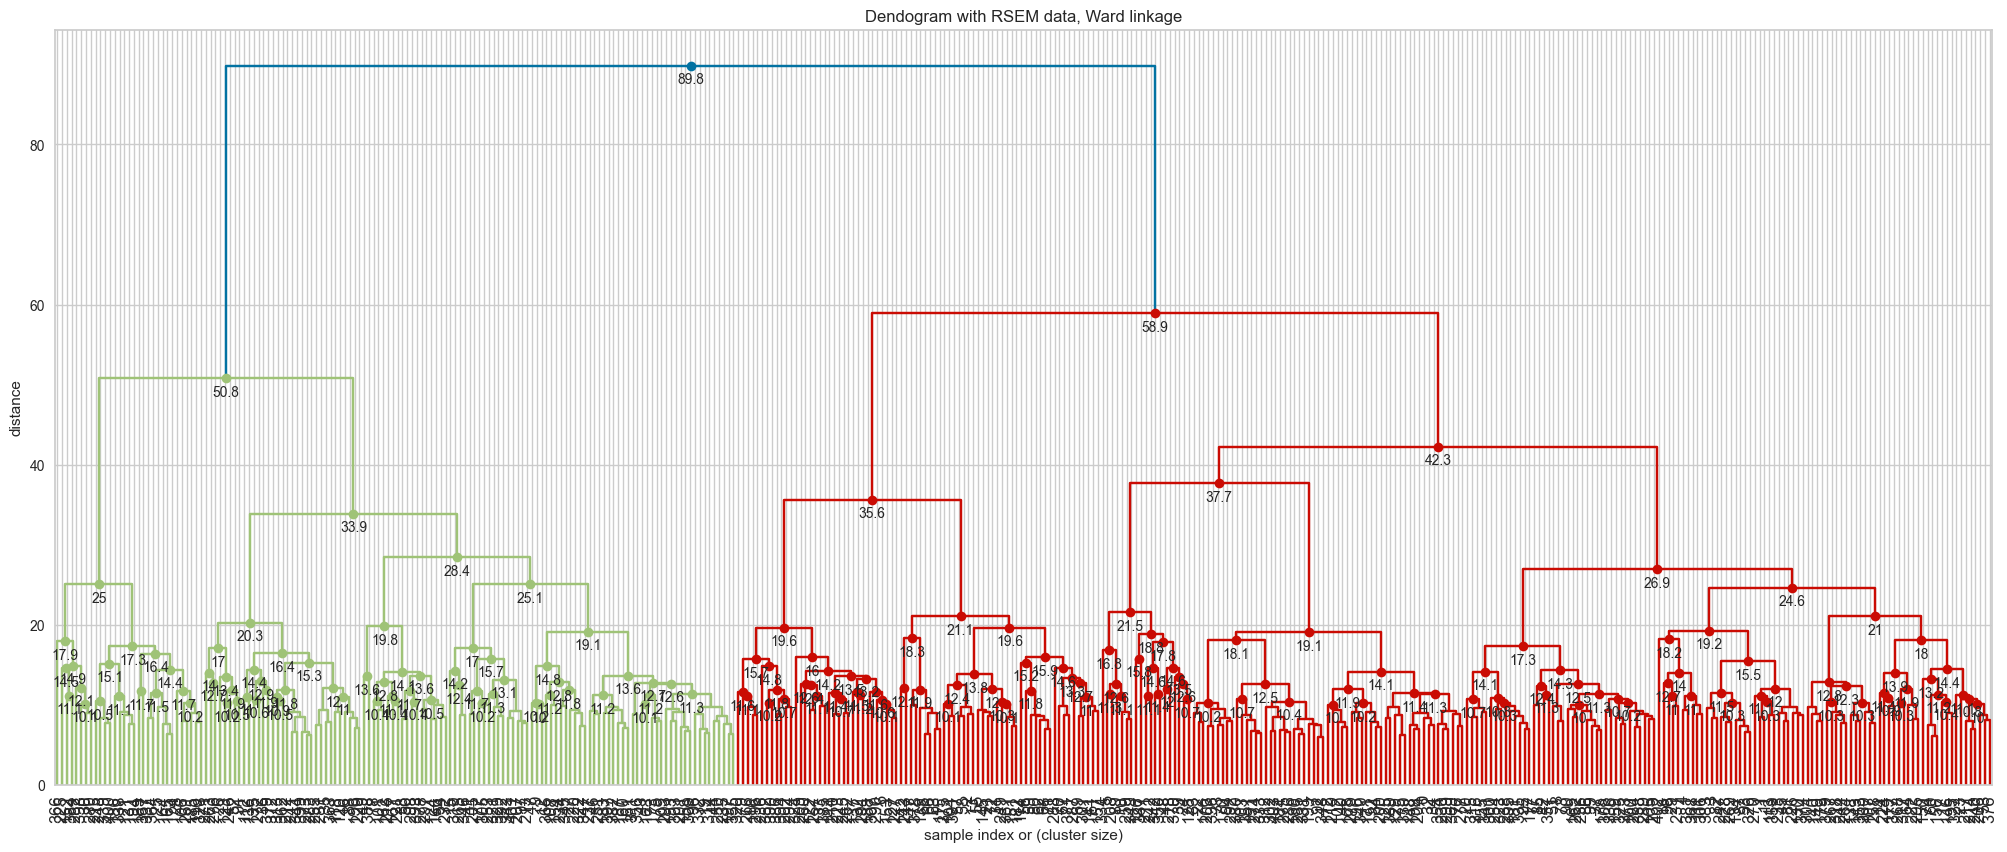
\includegraphics[width=1.0\textwidth,height=1.0\textheight,keepaspectratio]{Images/Clustering/dendogram.png}
%       \caption{Dendogram specific to hierarchical clustering and it can be seen how the algorithm starts classifying each datapoint in its own cluster followed by a merge in higher up clusters. For this we have used the TCGA dataset for bladder cancer, using hierarchical clsutering with Ward linkage.}
%       \label{fig:dendogram}
%   \end{figure}
%   \FloatBarrier





\section{Network I}

\subsection{Selective edge pruning} \label{s:ap:sel_prun}

% Comunity sizes
\begin{figure}[!h]
    \captionsetup[subfigure]{justification=Centering}
    \begin{subfigure}[!t]{0.5\textwidth}
        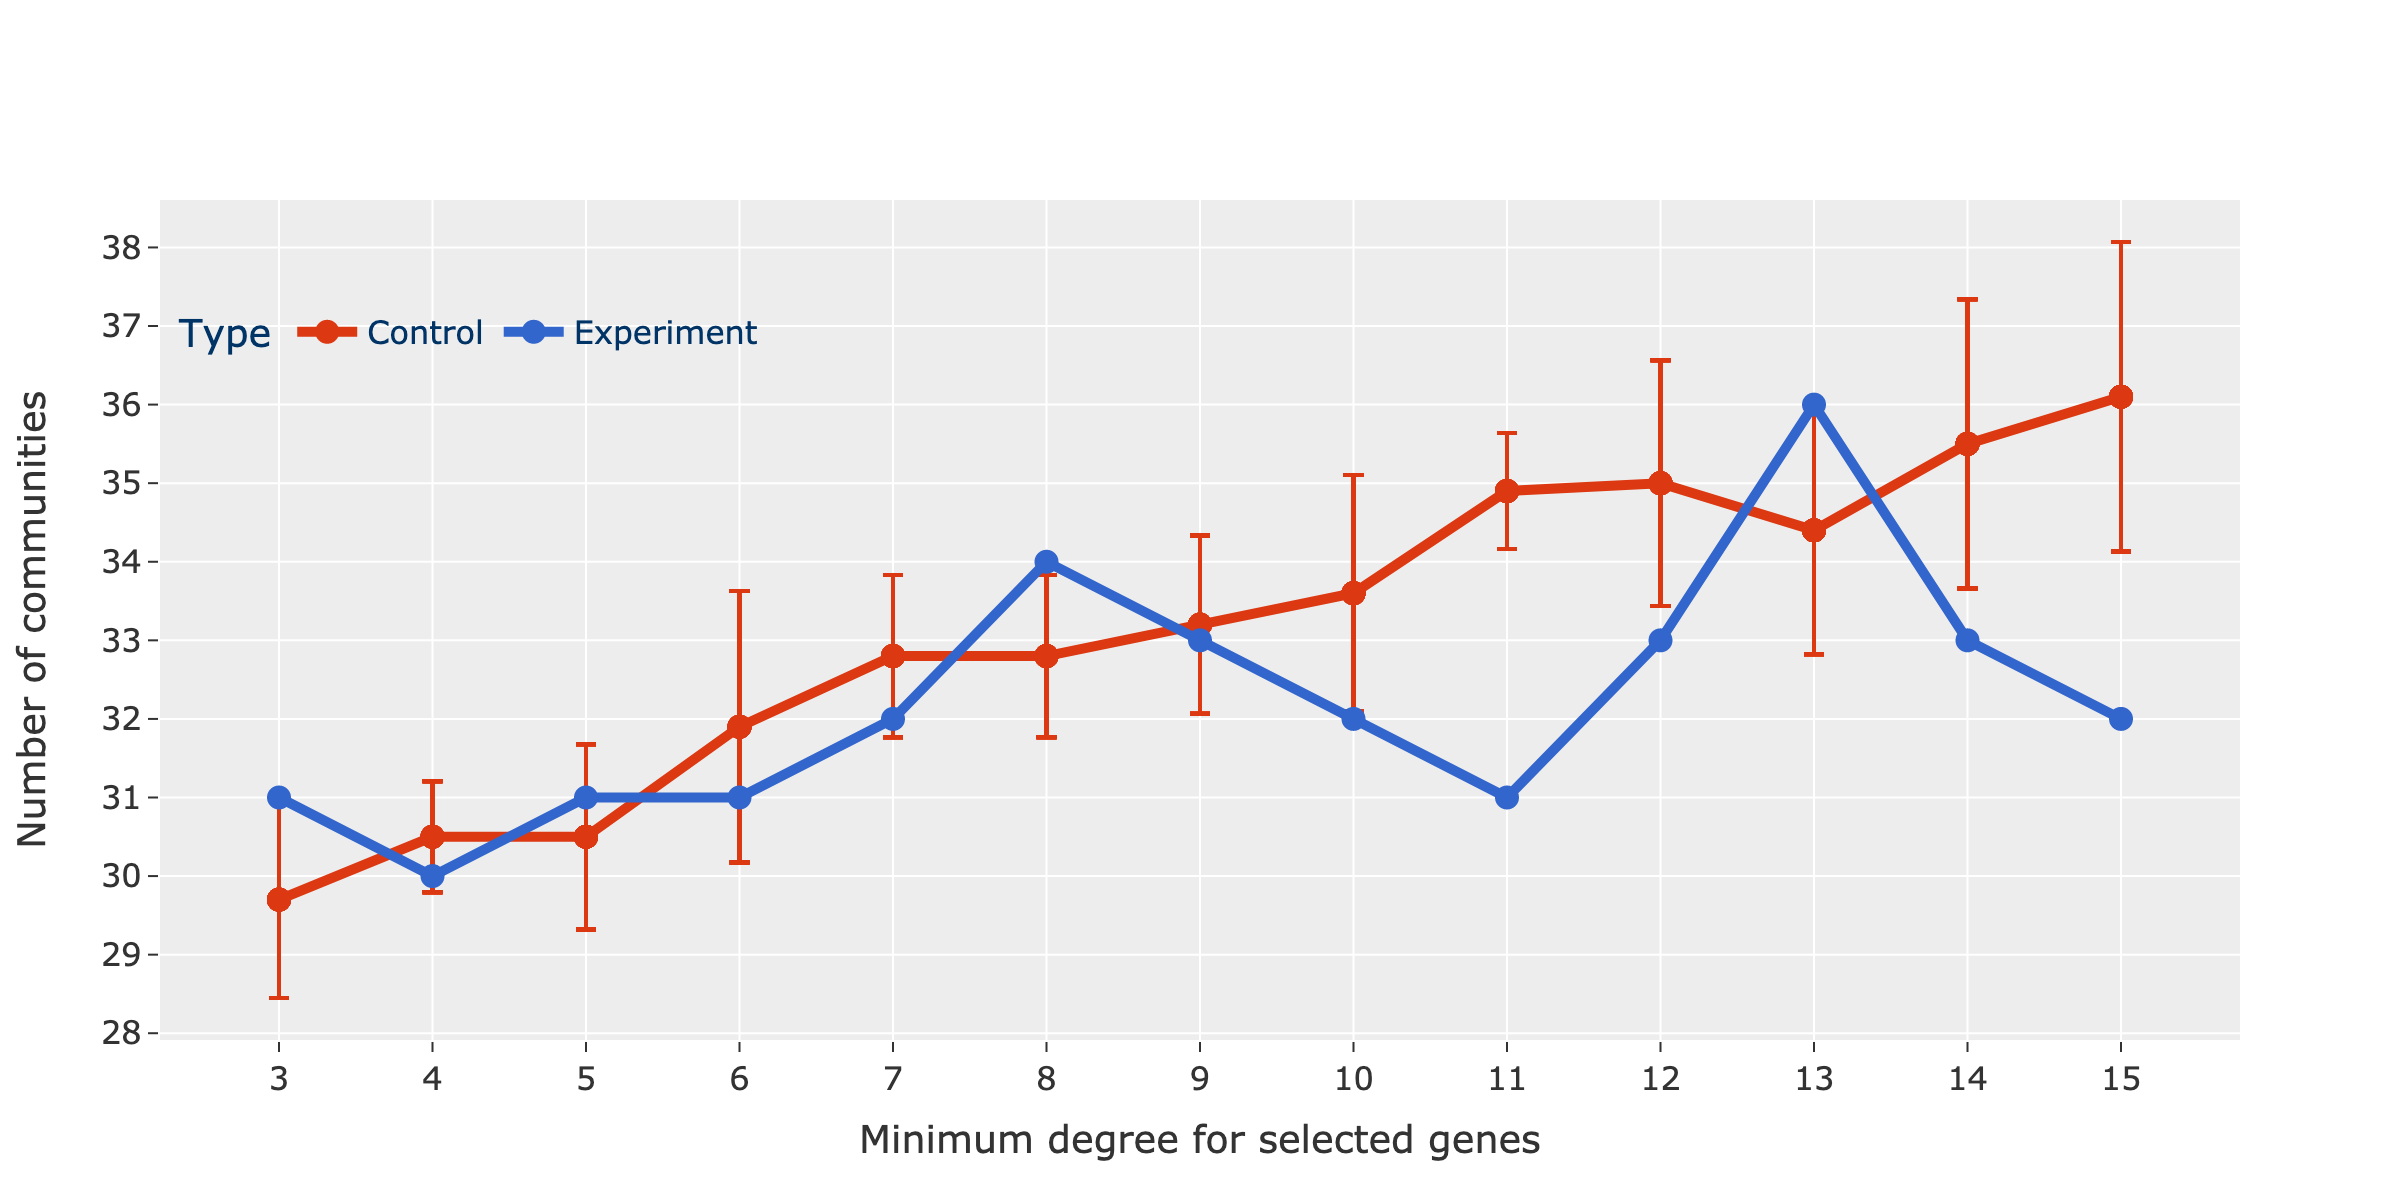
\includegraphics[width=\textwidth]{Sections/Network_I/Resources/selective_pruning/sbm_comNum_sel_prun.png}
        \caption{SBM}
        \label{fig:ap:sbm_com_size}
    \end{subfigure}\hspace{\fill} % maximize horizontal separation
    \begin{subfigure}[!t]{0.5\textwidth}
        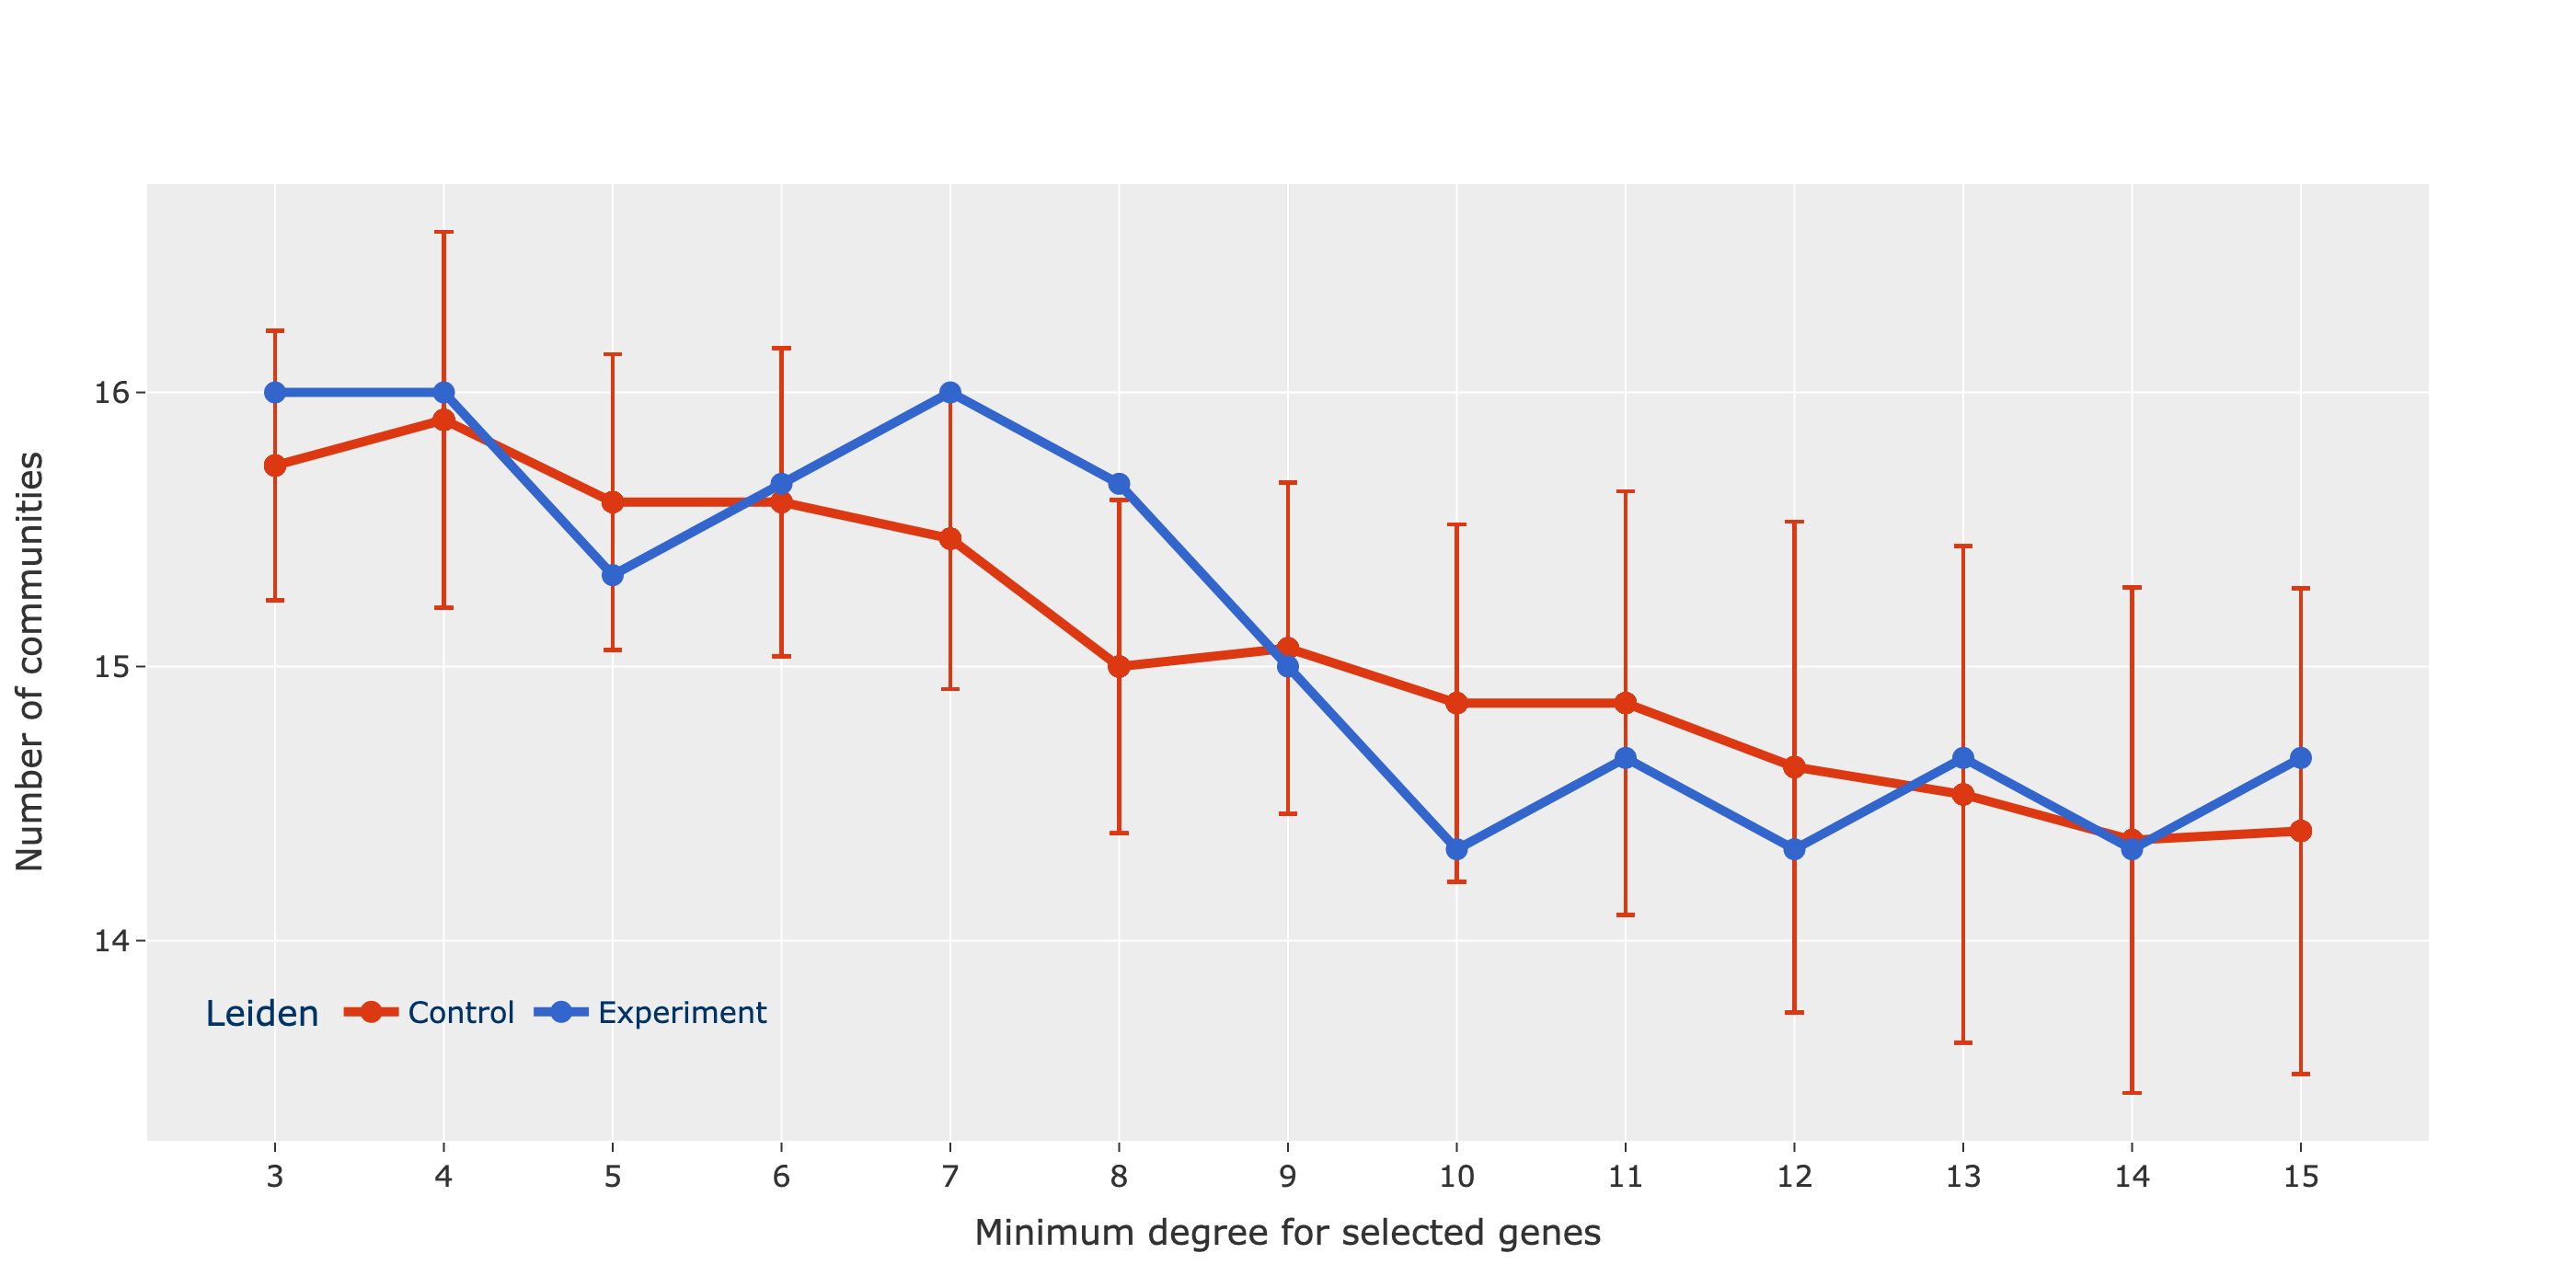
\includegraphics[width=\linewidth]{Sections/Network_I/Resources/selective_pruning/leid_comNum_sel_prun.png}
        \caption{Leiden}
            \label{fig:ap:leid_com_size}
    \end{subfigure}\hspace{\fill} % maximize horizontal separation

    \caption{Community size comparison between Leiden and SBM. This serves as a supporting material to the work done in \cref{s:N_I:sel_pruning}}
    \label{fig:ap:com_size_comp}
\end{figure}

%  Morpheus hierarchical clustering
\begin{figure}[H]   
\centering
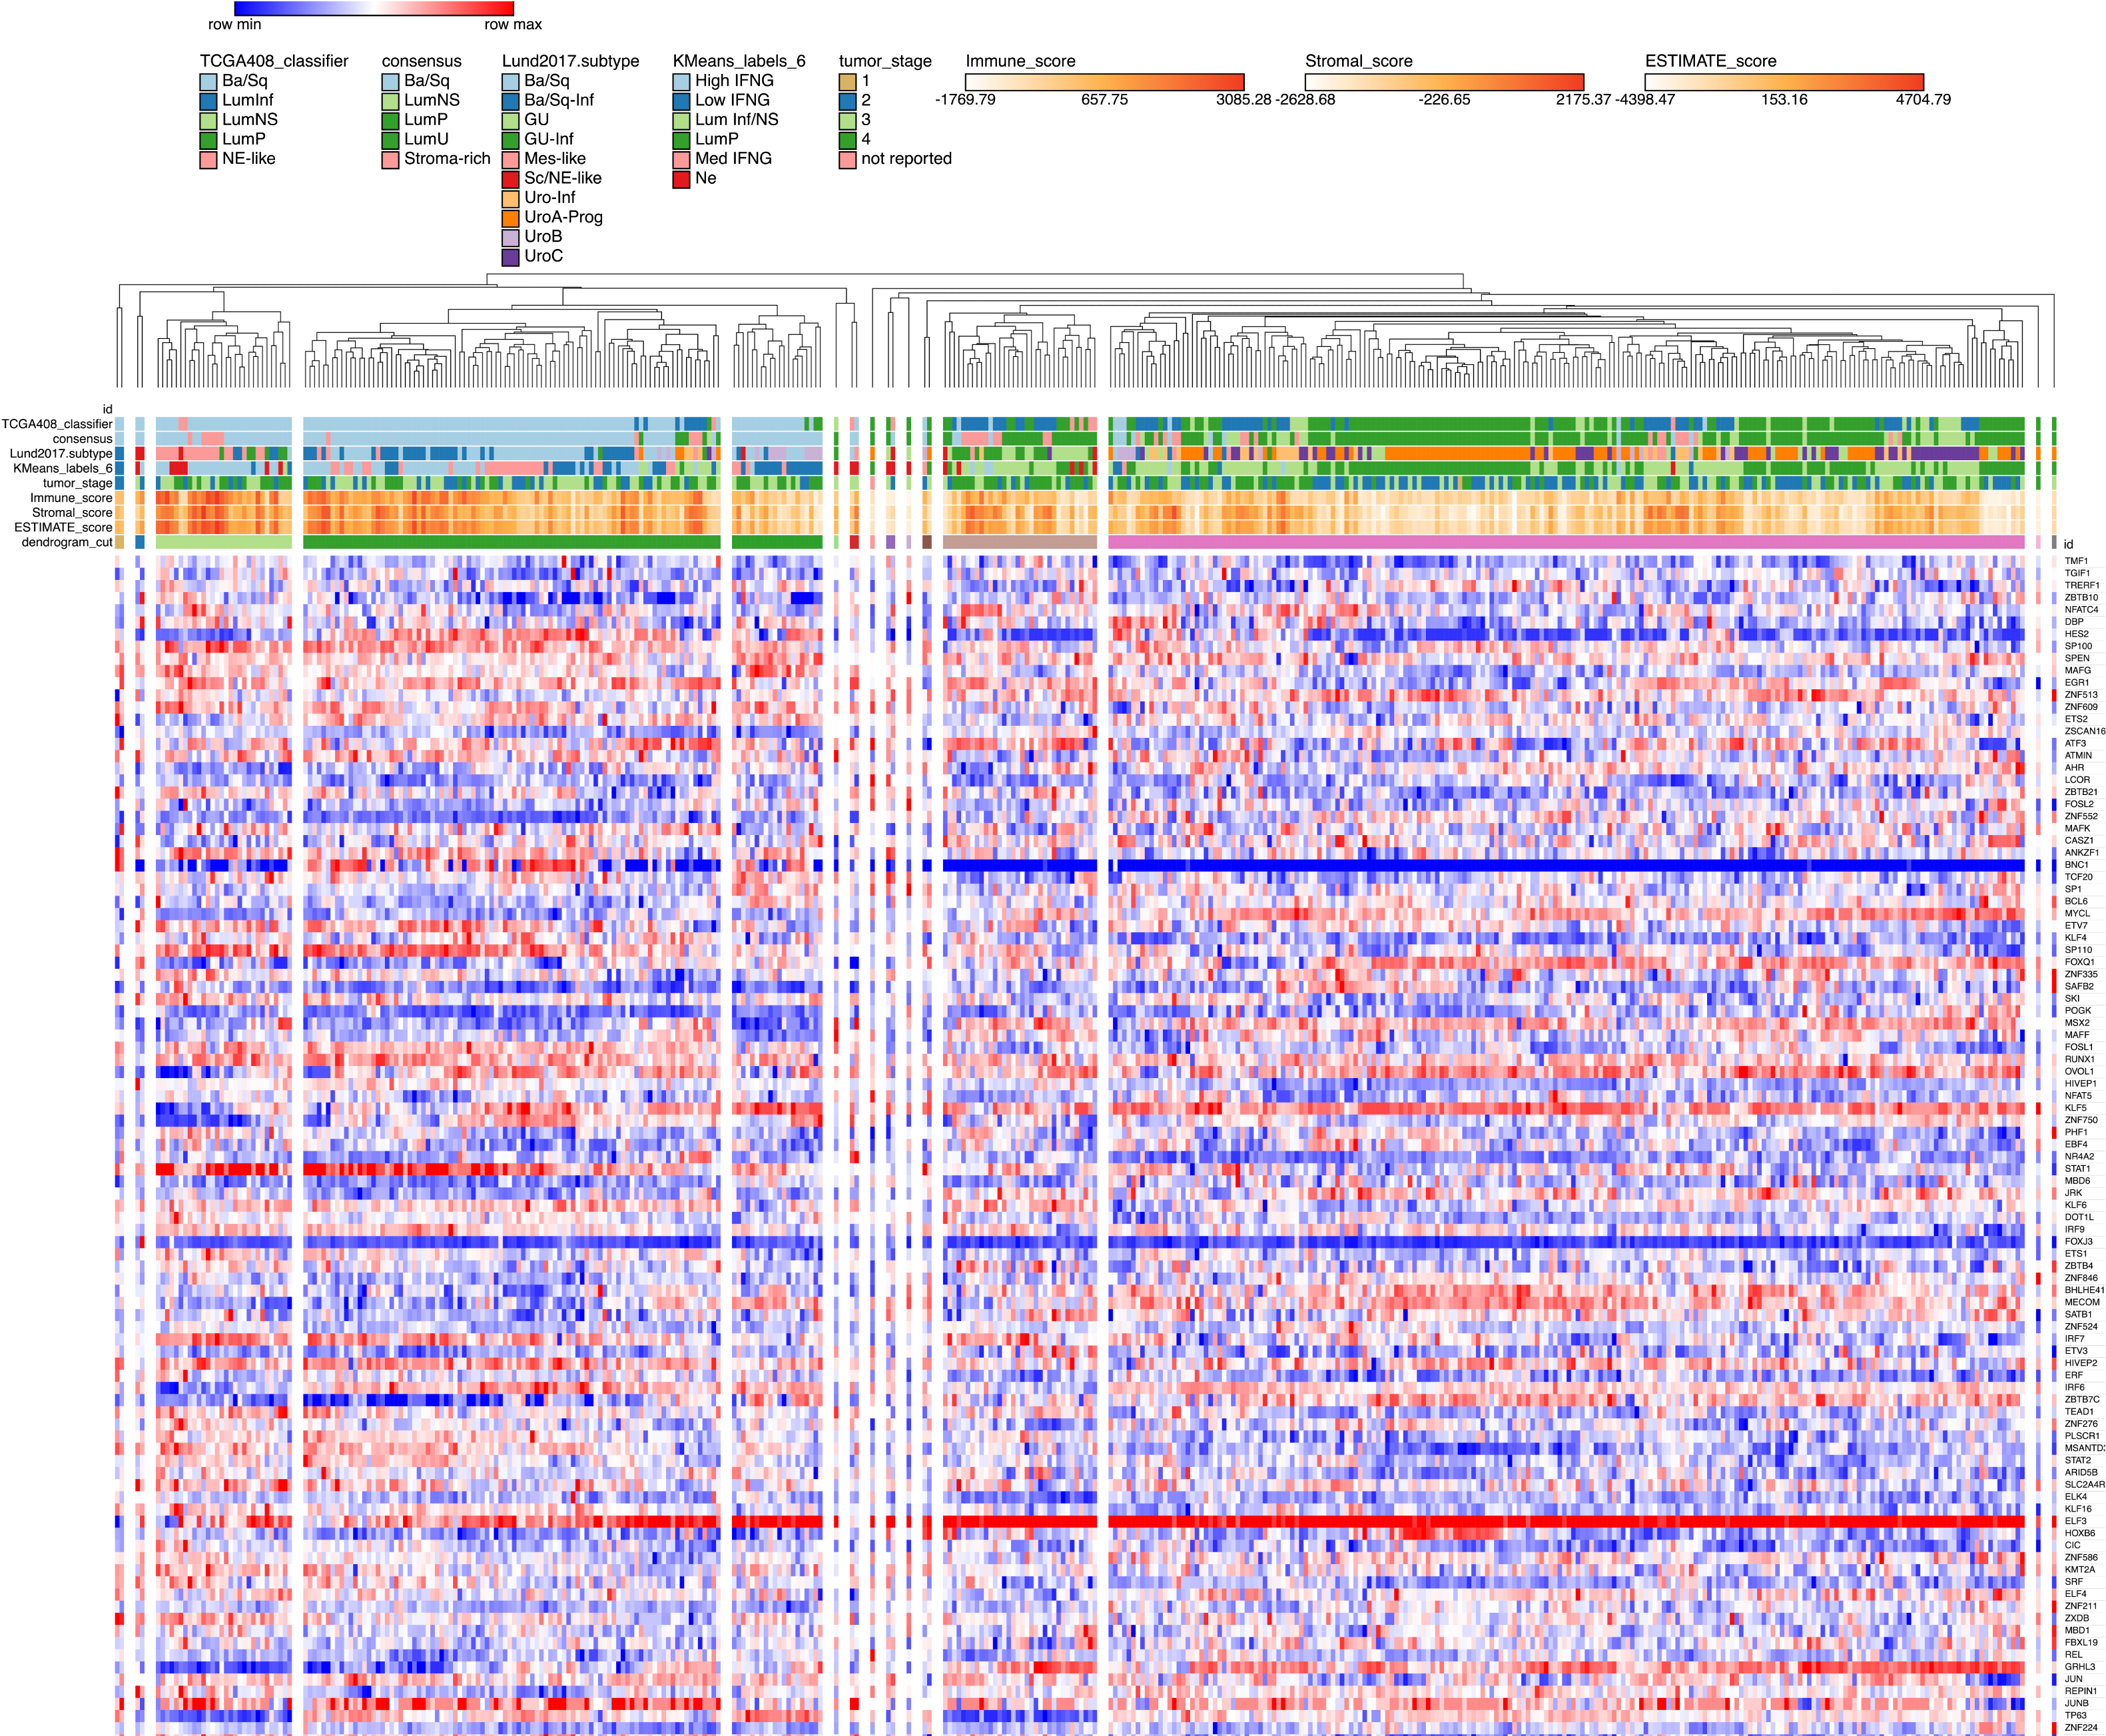
\includegraphics[width=1.0\textwidth,height=1.0\textheight,keepaspectratio]{Sections/Network_I/Resources/selective_pruning/15_CS_norm_sel_tfs.png}
  \caption{Hierarchical clustering of the 98 TFs found in \cref{s:sel_tfs}. The columns at the top of the heatmap represents the previous classification (TCGA \cite{Robertson2017-mg}, Consensus \cite{Kamoun2020-tj}, Lund \cite{Marzouka2018-ge} and the stratification from \cref{s:clustering_analysis}) as well as the Immune, Stromal and ESTIMATE scores available with the TCGA cohort.}
\label{fig:ap:morph_sel_tfs}
\end{figure}

\Cref{fig:N_I:sel_tfs_mean} depicts the mean expression of the 98 TFs genes found in the previous subsection. The log plot shows the non-cancerous mean on the y-axis and the tumour mean expression on the x-axis, the size and colour of the points is proportional to the mutation burden across the MIBC cohort from TCGA. The genes higher on the y-axis have a higher expression in the non-cancerous, similarly for x-axis, further on the right hand side, higher average value in the tumour cohort. \textit{ELF3} it is on the top right corner meaning that it is expressed both in the tumour and non-cancerous datasets, and it is also highly mutated in MIBC. \textit{BNC1} is on he left corner, having lower expression across the samples.

% Tum vs non-cancerous dataset.
\begin{figure}[H]   
\centering
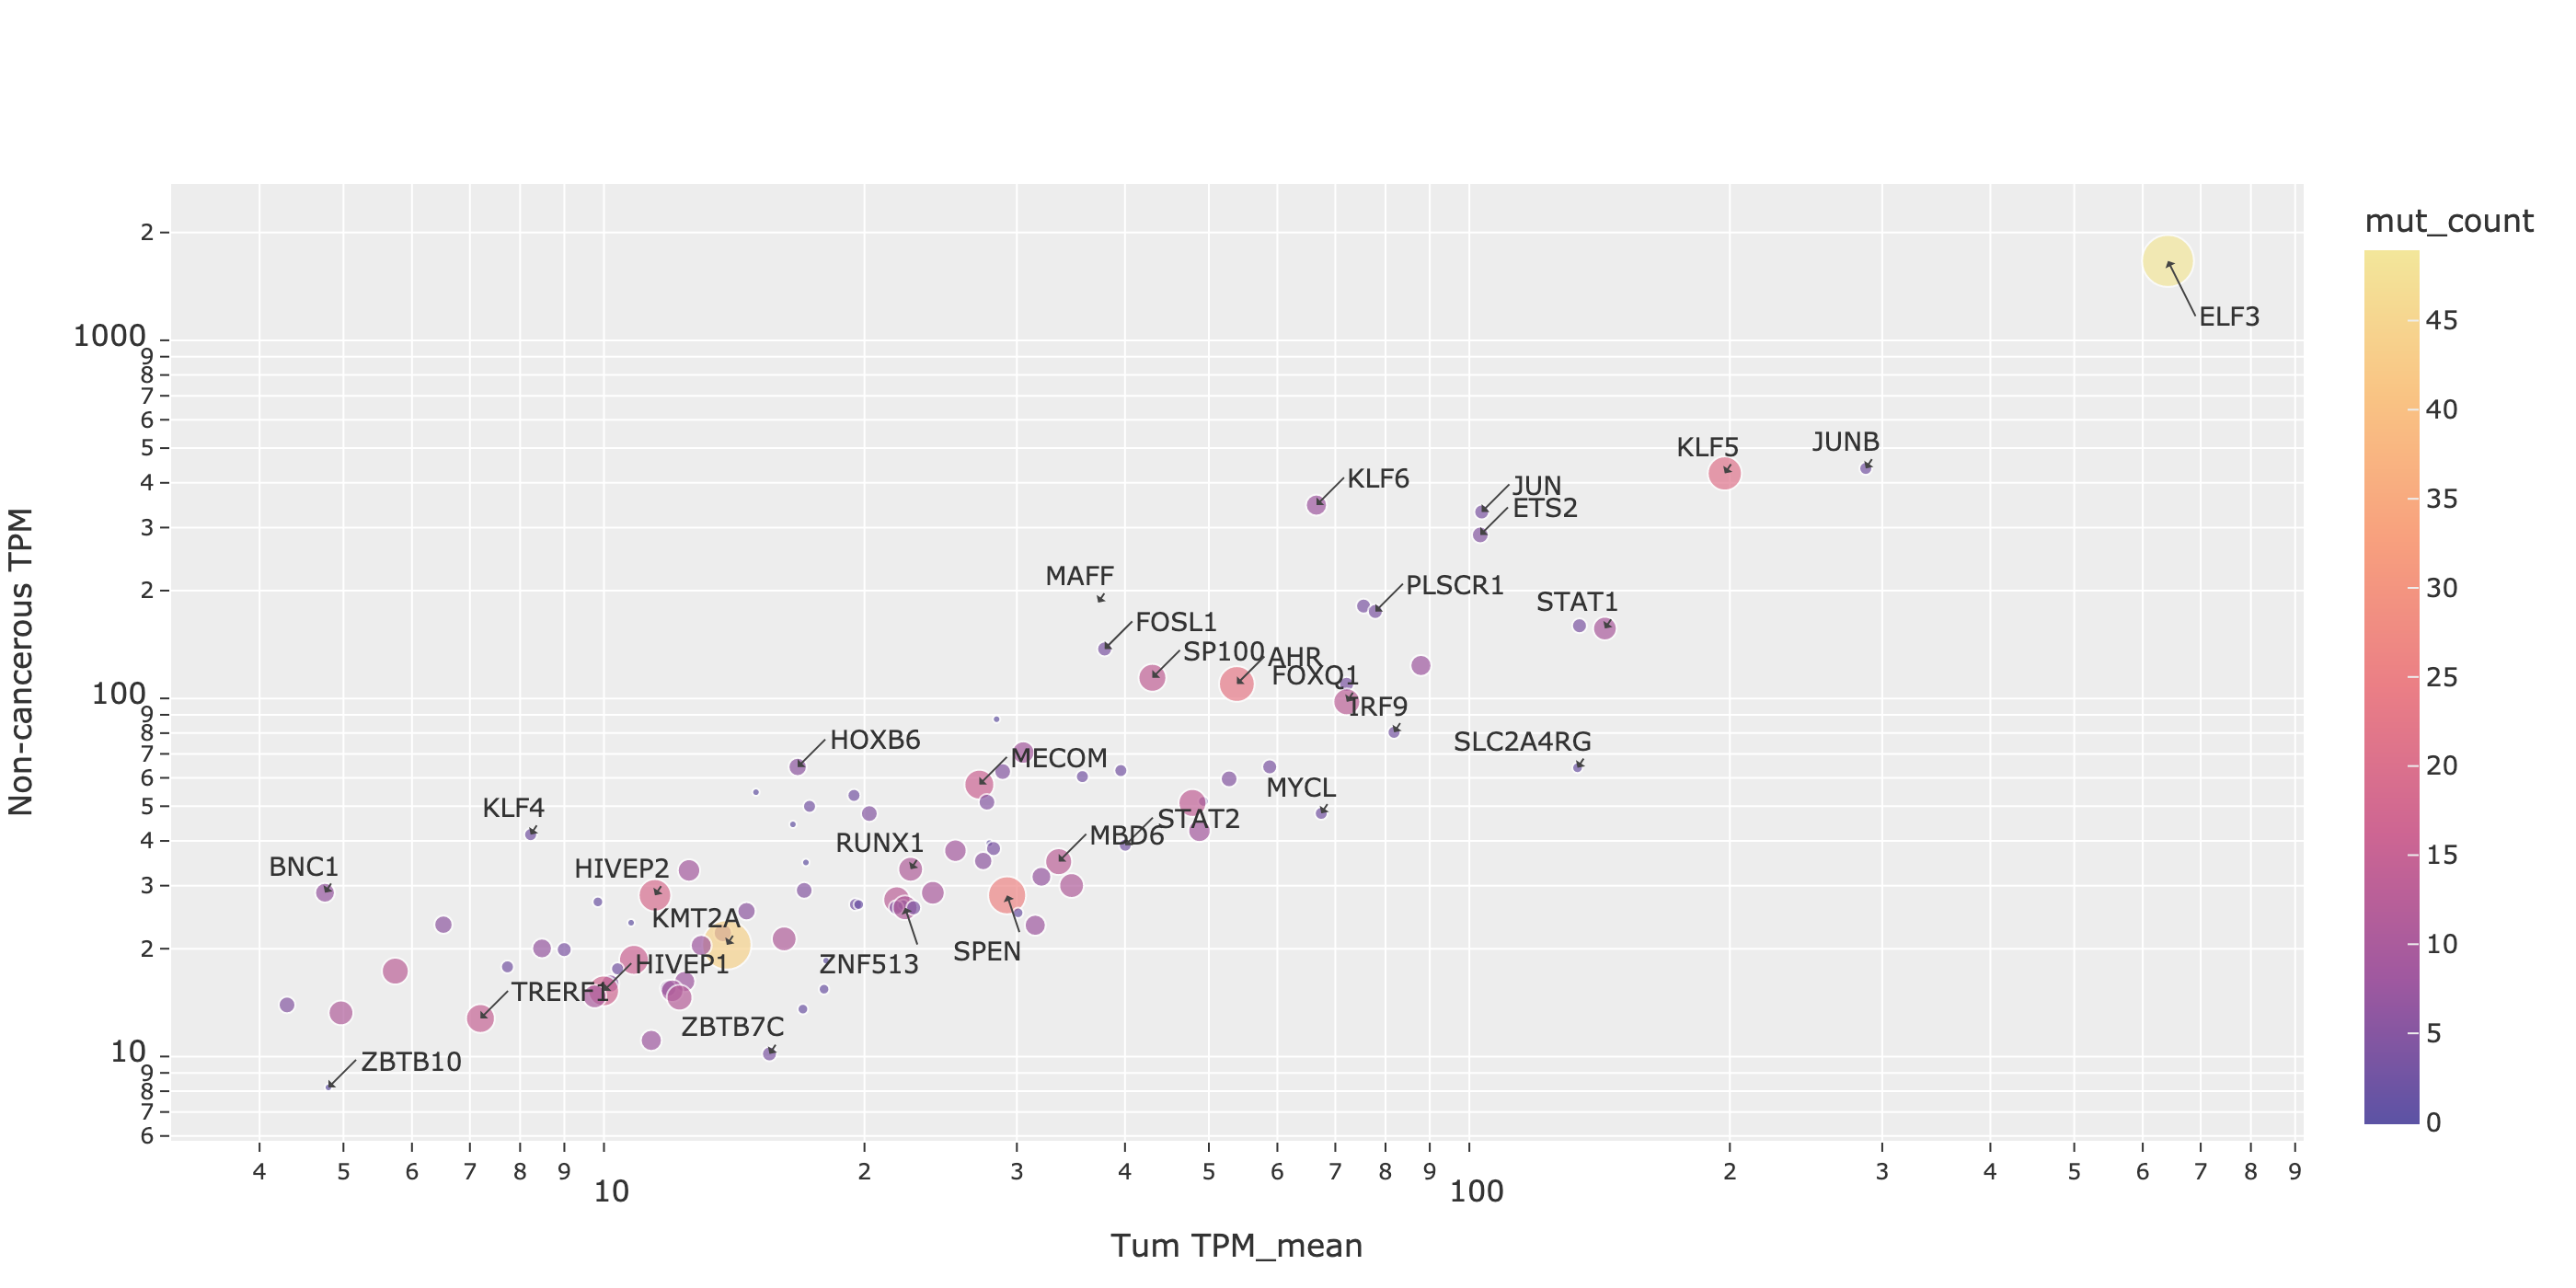
\includegraphics[width=1.0\textwidth,height=1.0\textheight,keepaspectratio]{Sections/Network_I/Resources/selective_pruning/sel_tfs_mean_tum_healthy.png}
  \caption{Selected TFs expression in the MIBC TCGA cohort and in the non-cancerous. Both the colour and size of the points are proportional to the mutation burden in the TCGA cohort.}
\label{fig:ap:sel_tfs_mean}
\end{figure}

% Metadata of the hierarchical clustering
\subsubsection{TCGA metadata and the clusters based on the 98 TFs} 

\label{s:ap:sel_prun_tcga_meta}

\begin{figure}[!htb]   
\centering
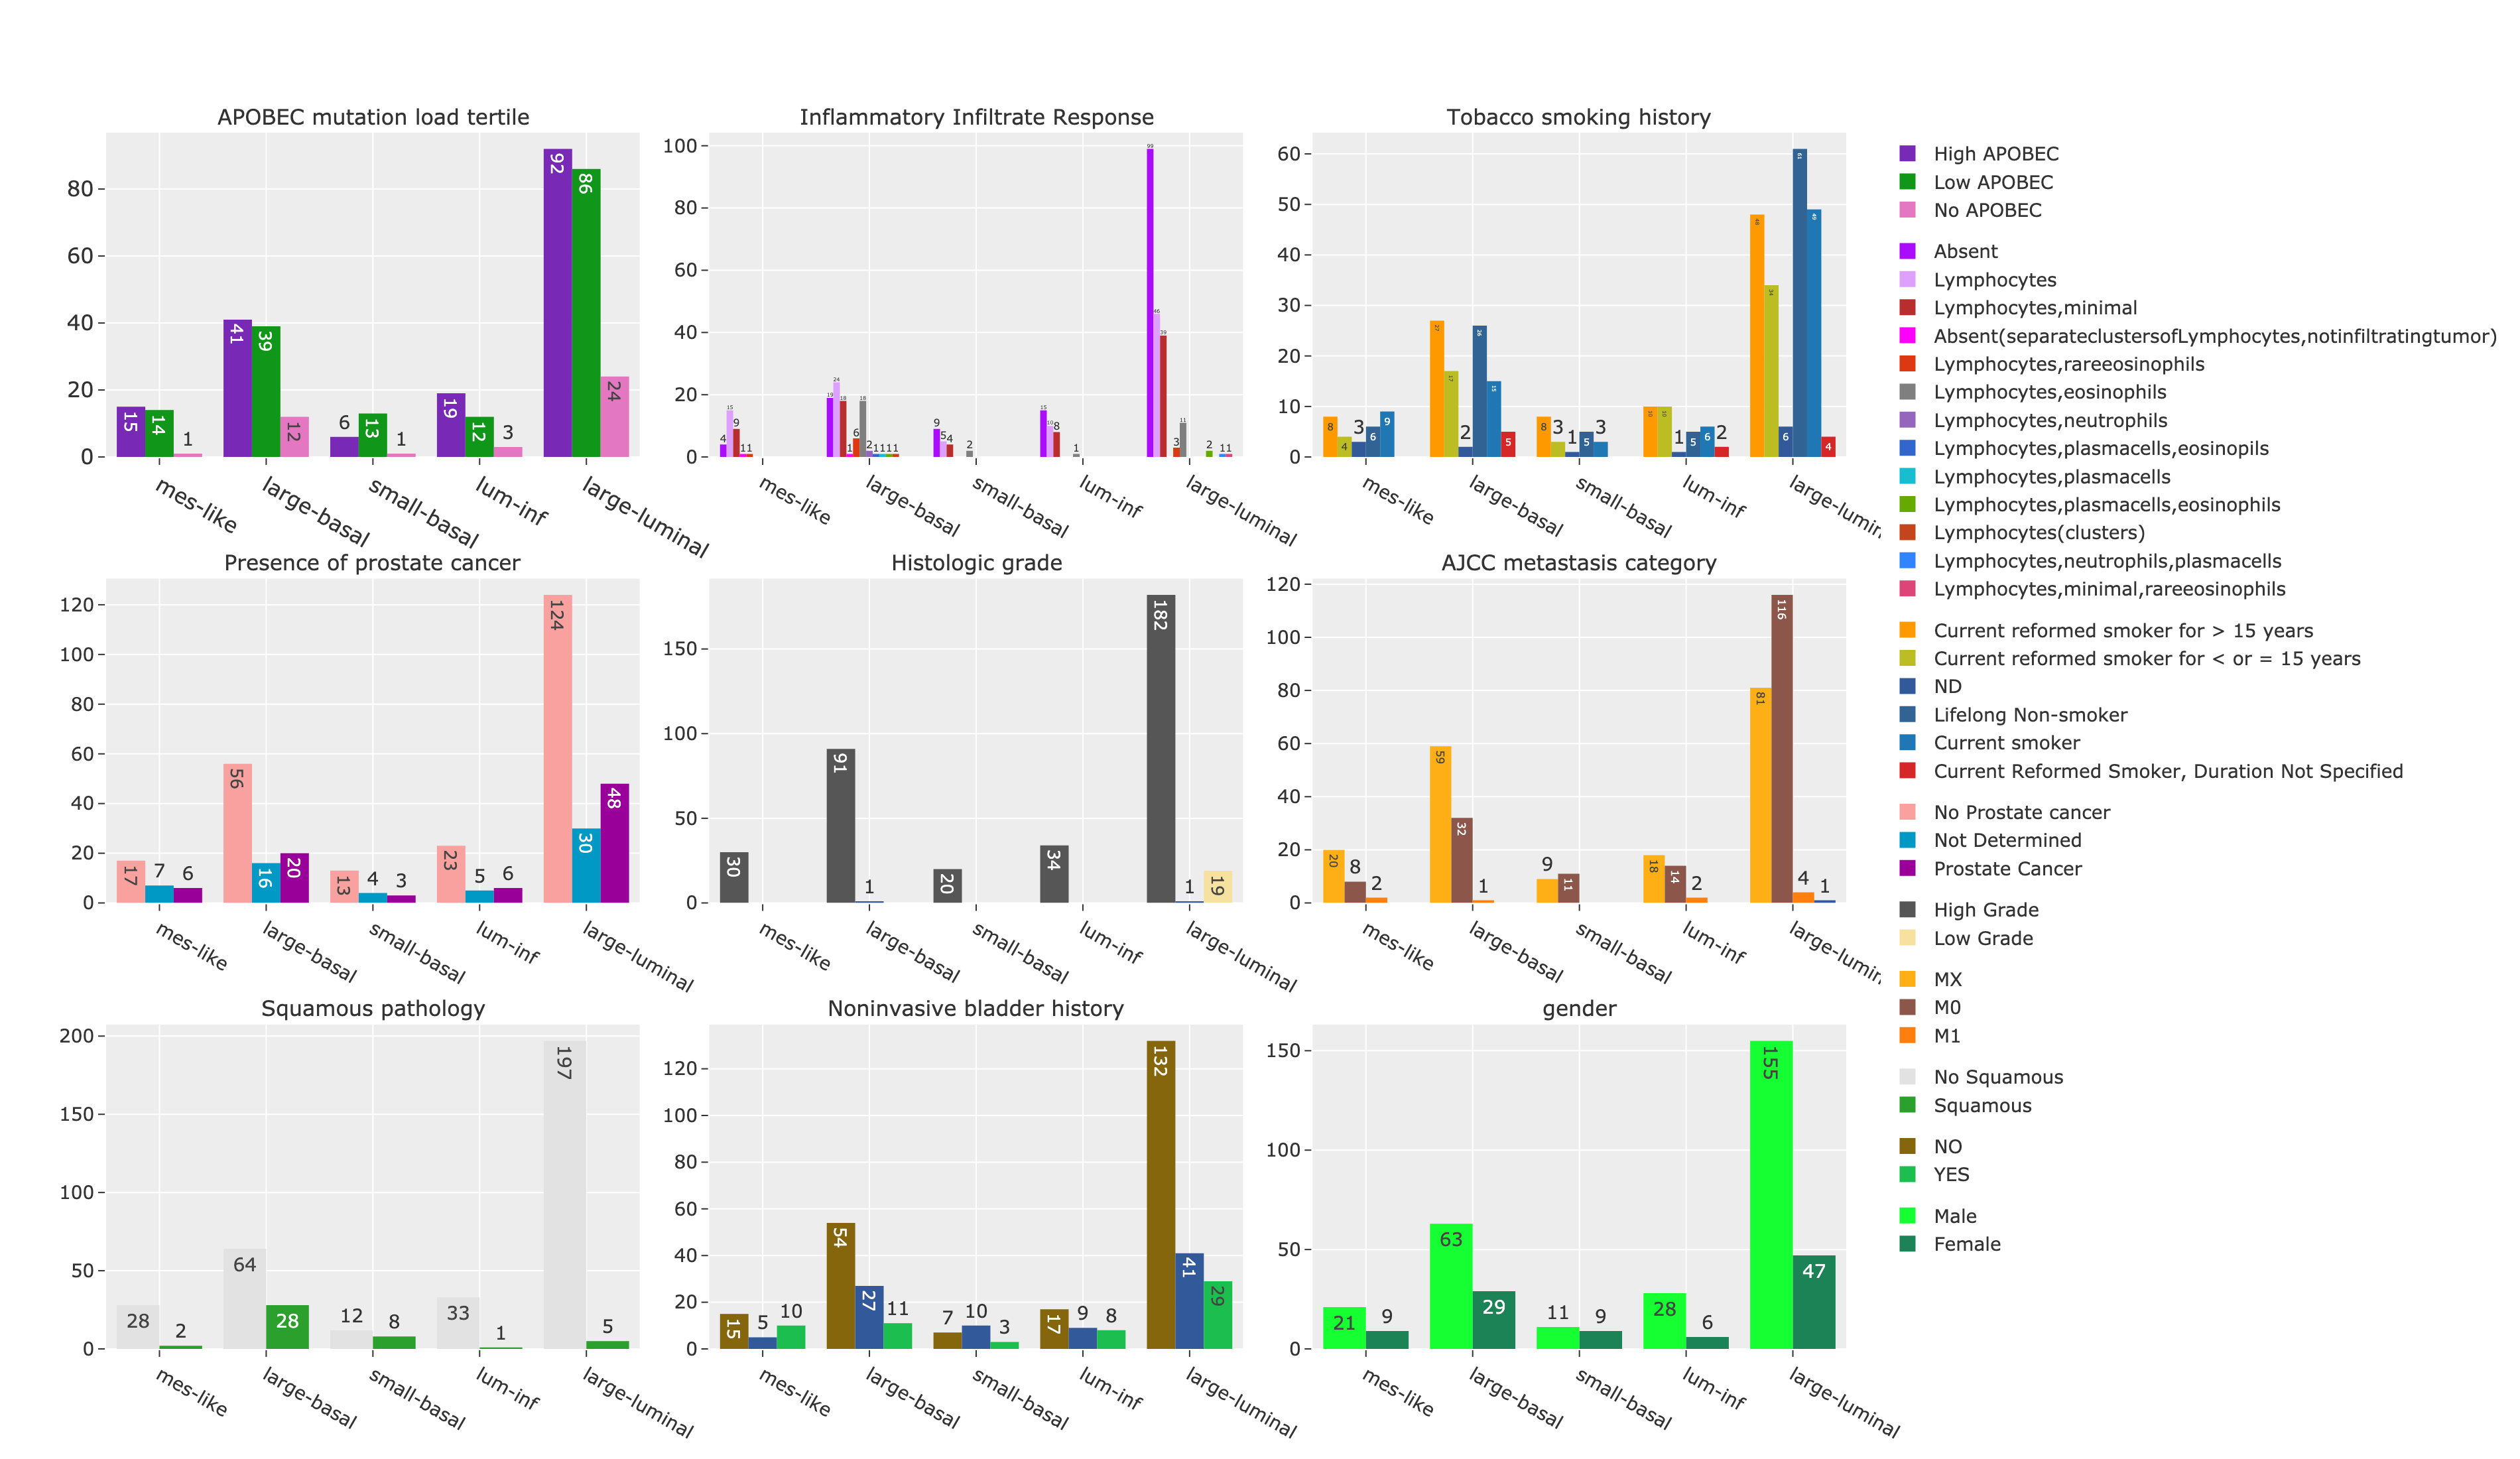
\includegraphics[width=1.0\textwidth,height=1.0\textheight,keepaspectratio]{Sections/Network_I/Resources/selective_pruning/sel_tfs_tcga_meta.png}
  \caption{The metadata from TCGA \cite{Robertson2017-mg} across the subtypes derived from applying hierarchical clustering on the expression of the 98 TFs from \cref{fig:N_I:sel_tfs}. }
\label{fig:ap:sel_tfs_tcga_metadata}
\end{figure}

\begin{figure}[!htb]   
\centering
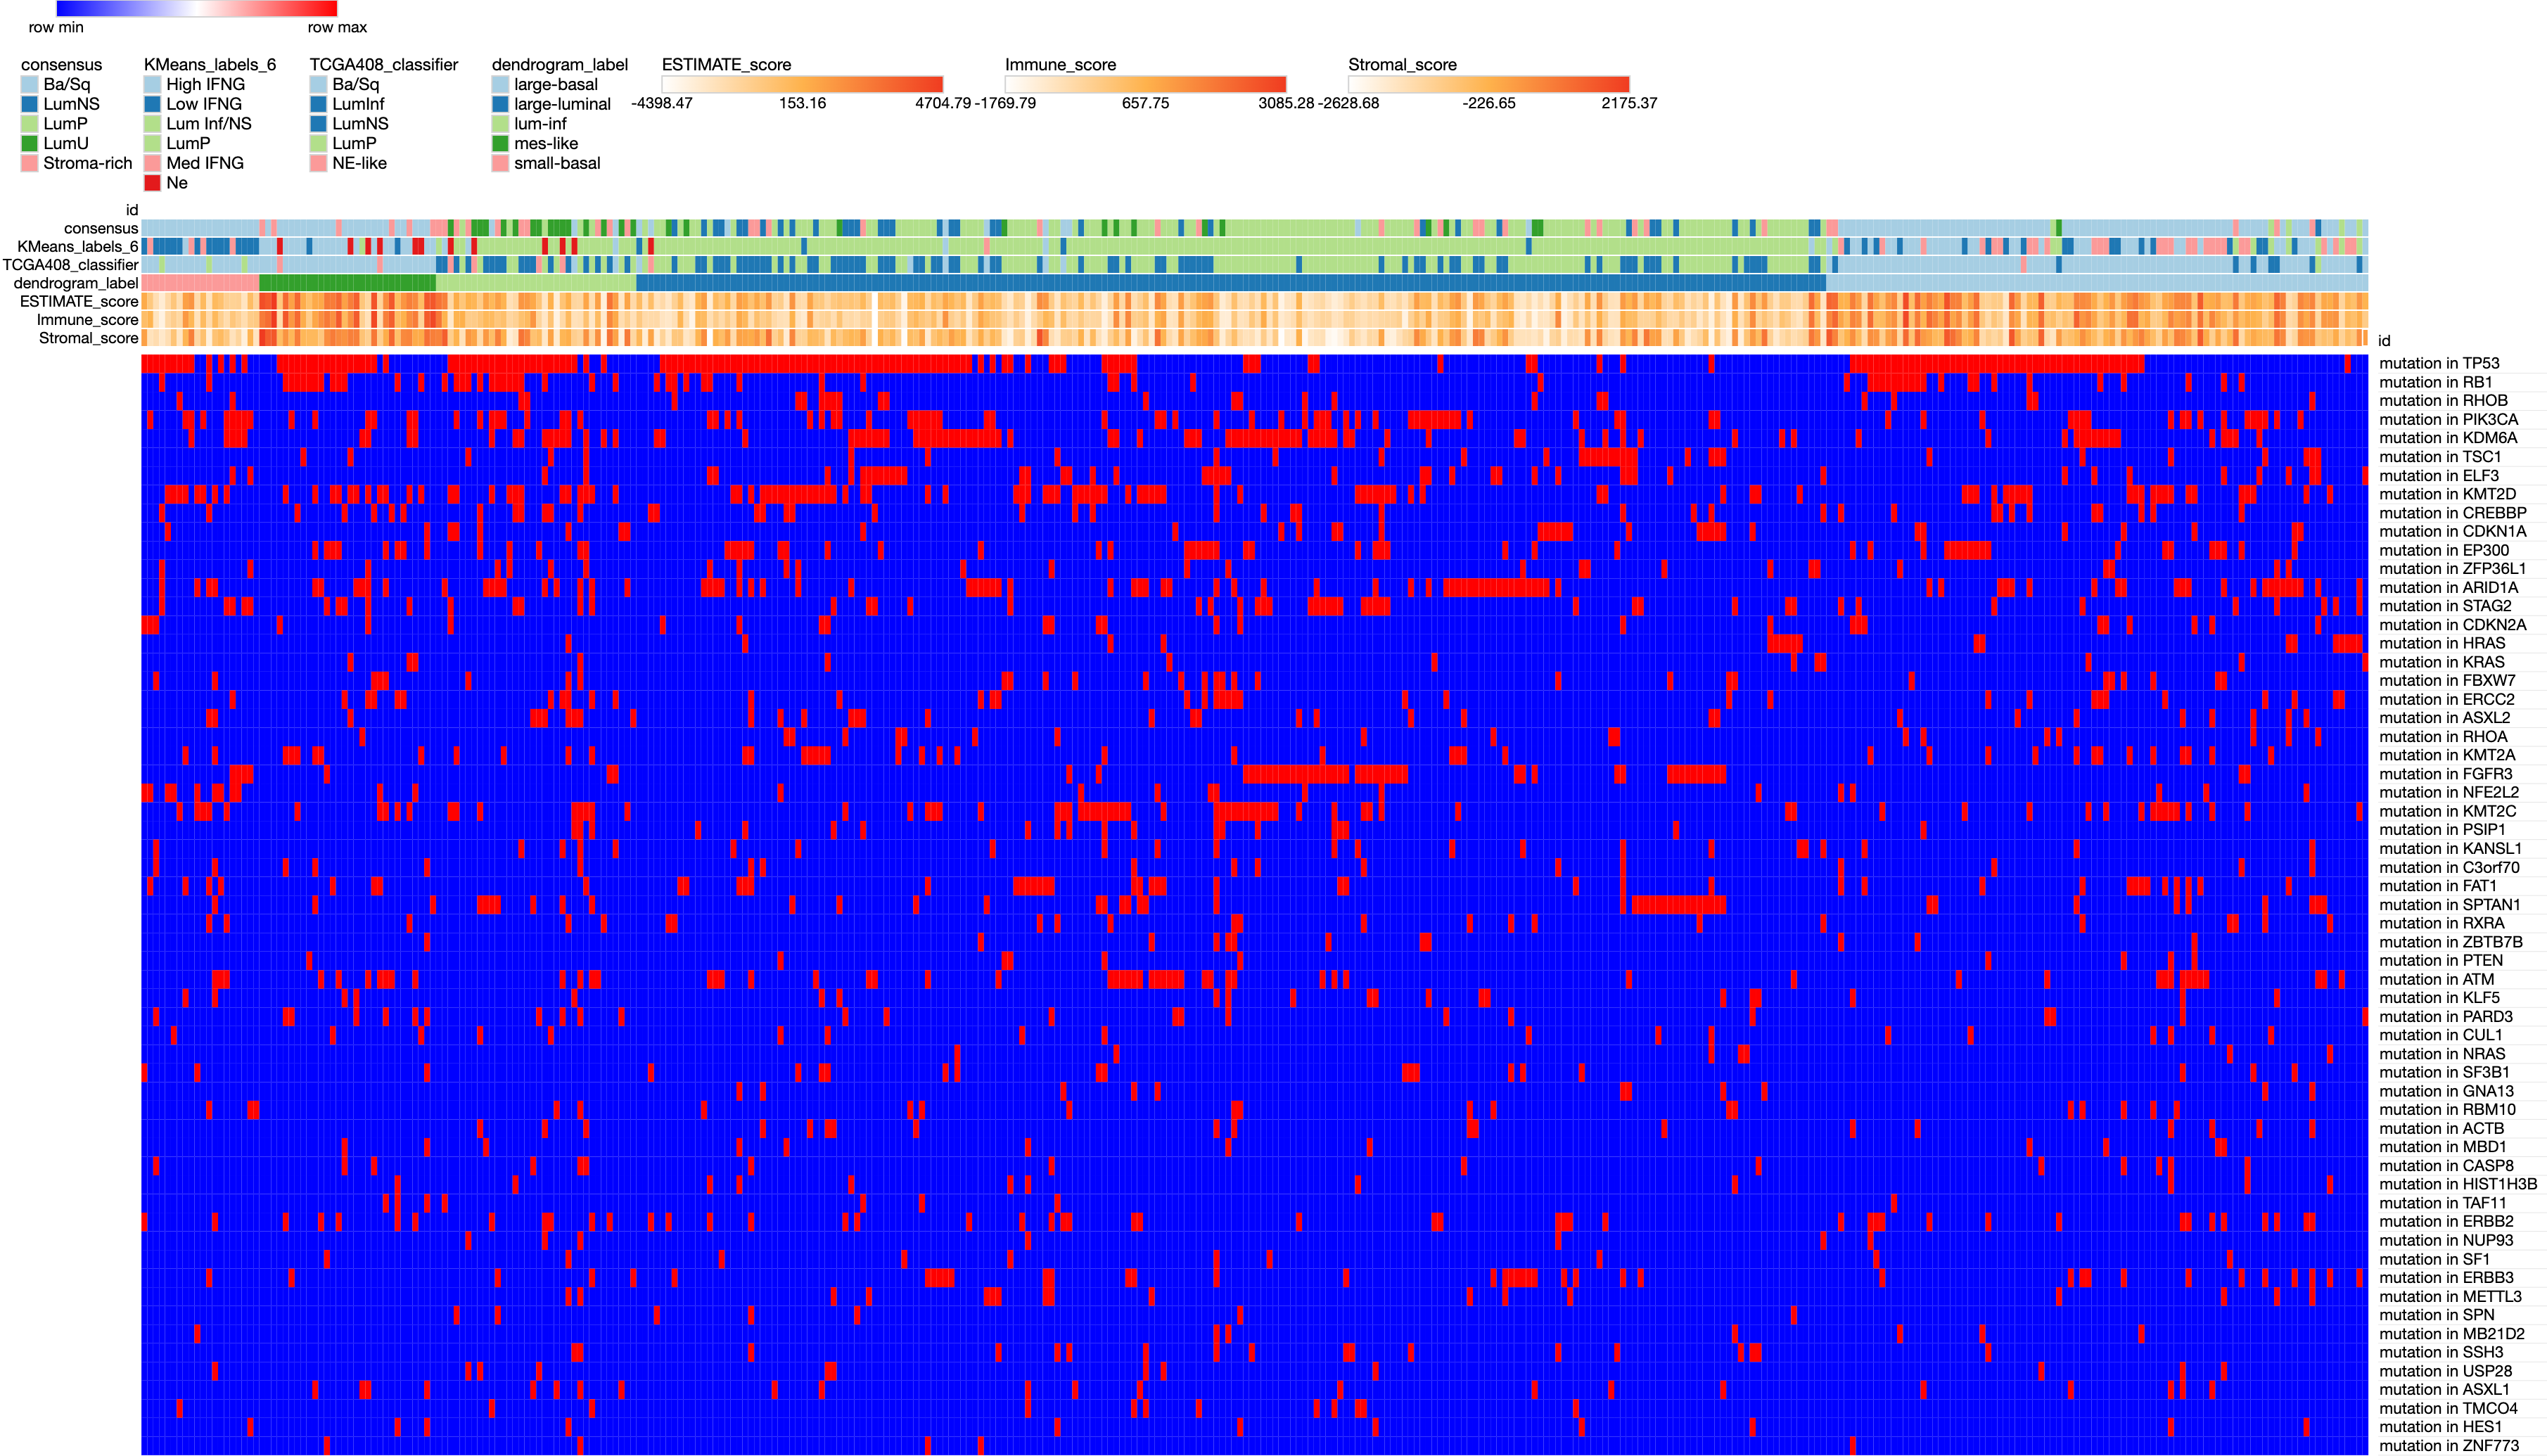
\includegraphics[width=1.0\textwidth,height=1.0\textheight,keepaspectratio]{Sections/Network_I/Resources/selective_pruning/sel_tfs_mut_meta.png}
  \caption{Heatmap of binary somatic mutation across.}
\label{fig:ap:sel_tfs_tcga_meta_mut}
\end{figure}

\begin{figure}[!htb]   
\centering
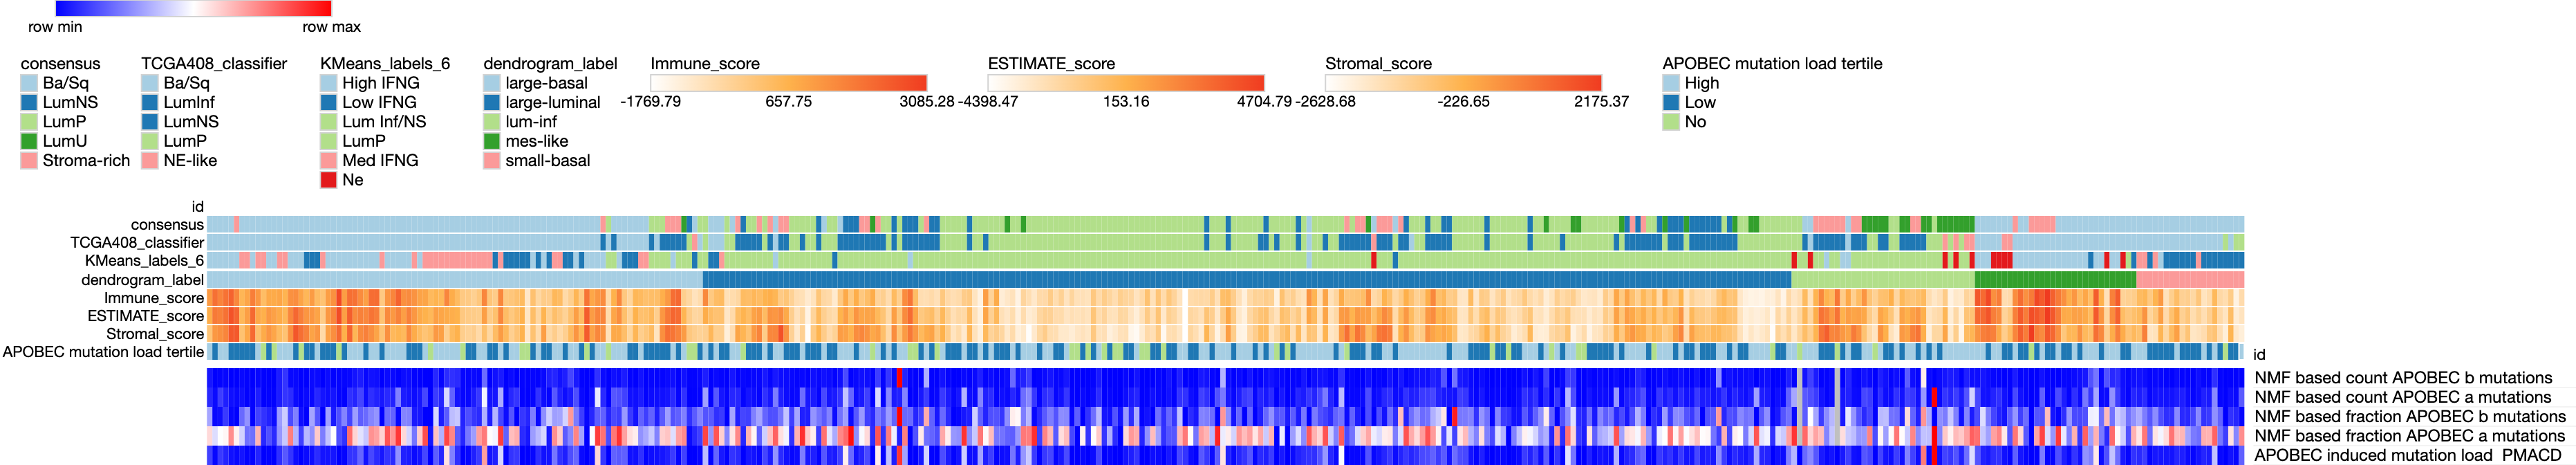
\includegraphics[width=1.0\textwidth,height=1.0\textheight,keepaspectratio]{Sections/Network_I/Resources/selective_pruning/sel_tfs_apobec_meta.png}
  \caption{Heatmap of the the APOBEC mutations in TCGA.}
\label{fig:ap:sel_tfs_tcga_meta_apobec}
\end{figure}





% Pi-plots for GSEA
\subsubsection{Pi-plots for GSEA} \label{s:ap:sel_prun_pi}

\begin{figure}[!h]
    \captionsetup[subfigure]{justification=Centering}
    \begin{subfigure}[!t]{0.9\linewidth}
        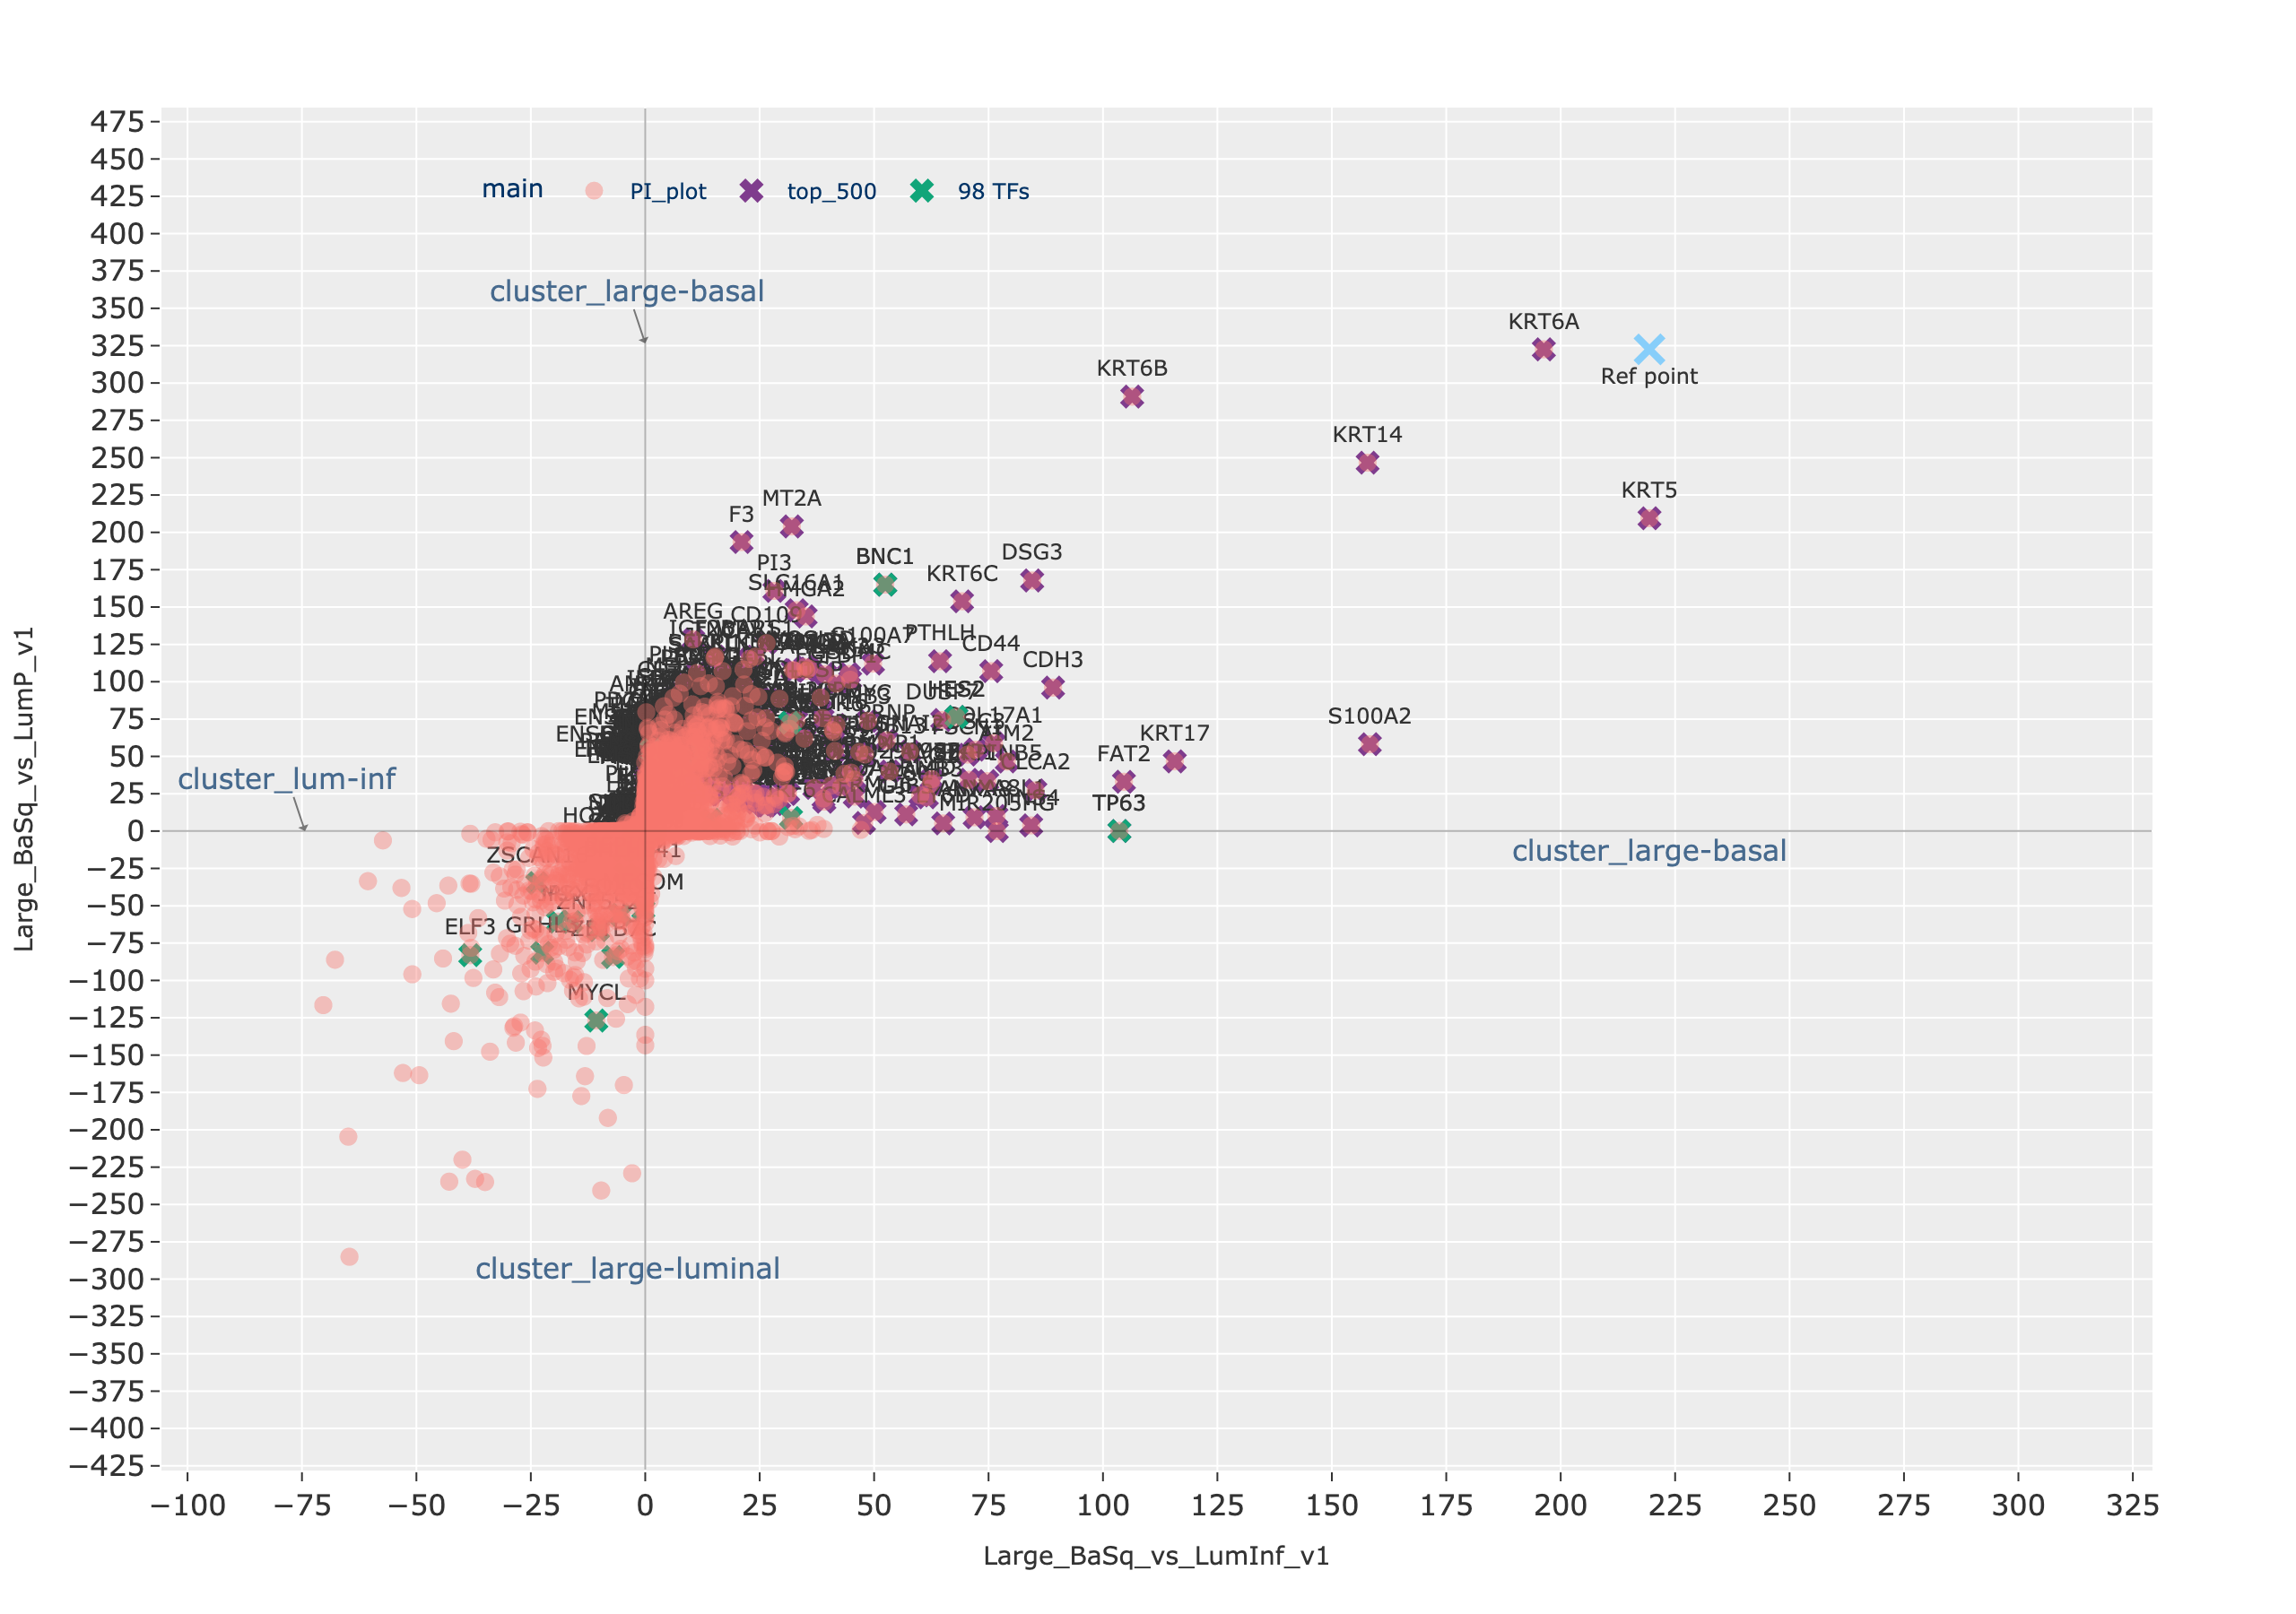
\includegraphics[width=\textwidth,keepaspectratio]{Sections/Network_I/Resources/selective_pruning/pi_gsea/pi_largeBasal.png}
        \caption{Large Basal}
    \end{subfigure}\hspace{\fill} % maximize horizontal separation
    \begin{subfigure}[!t]{0.9\textwidth}
        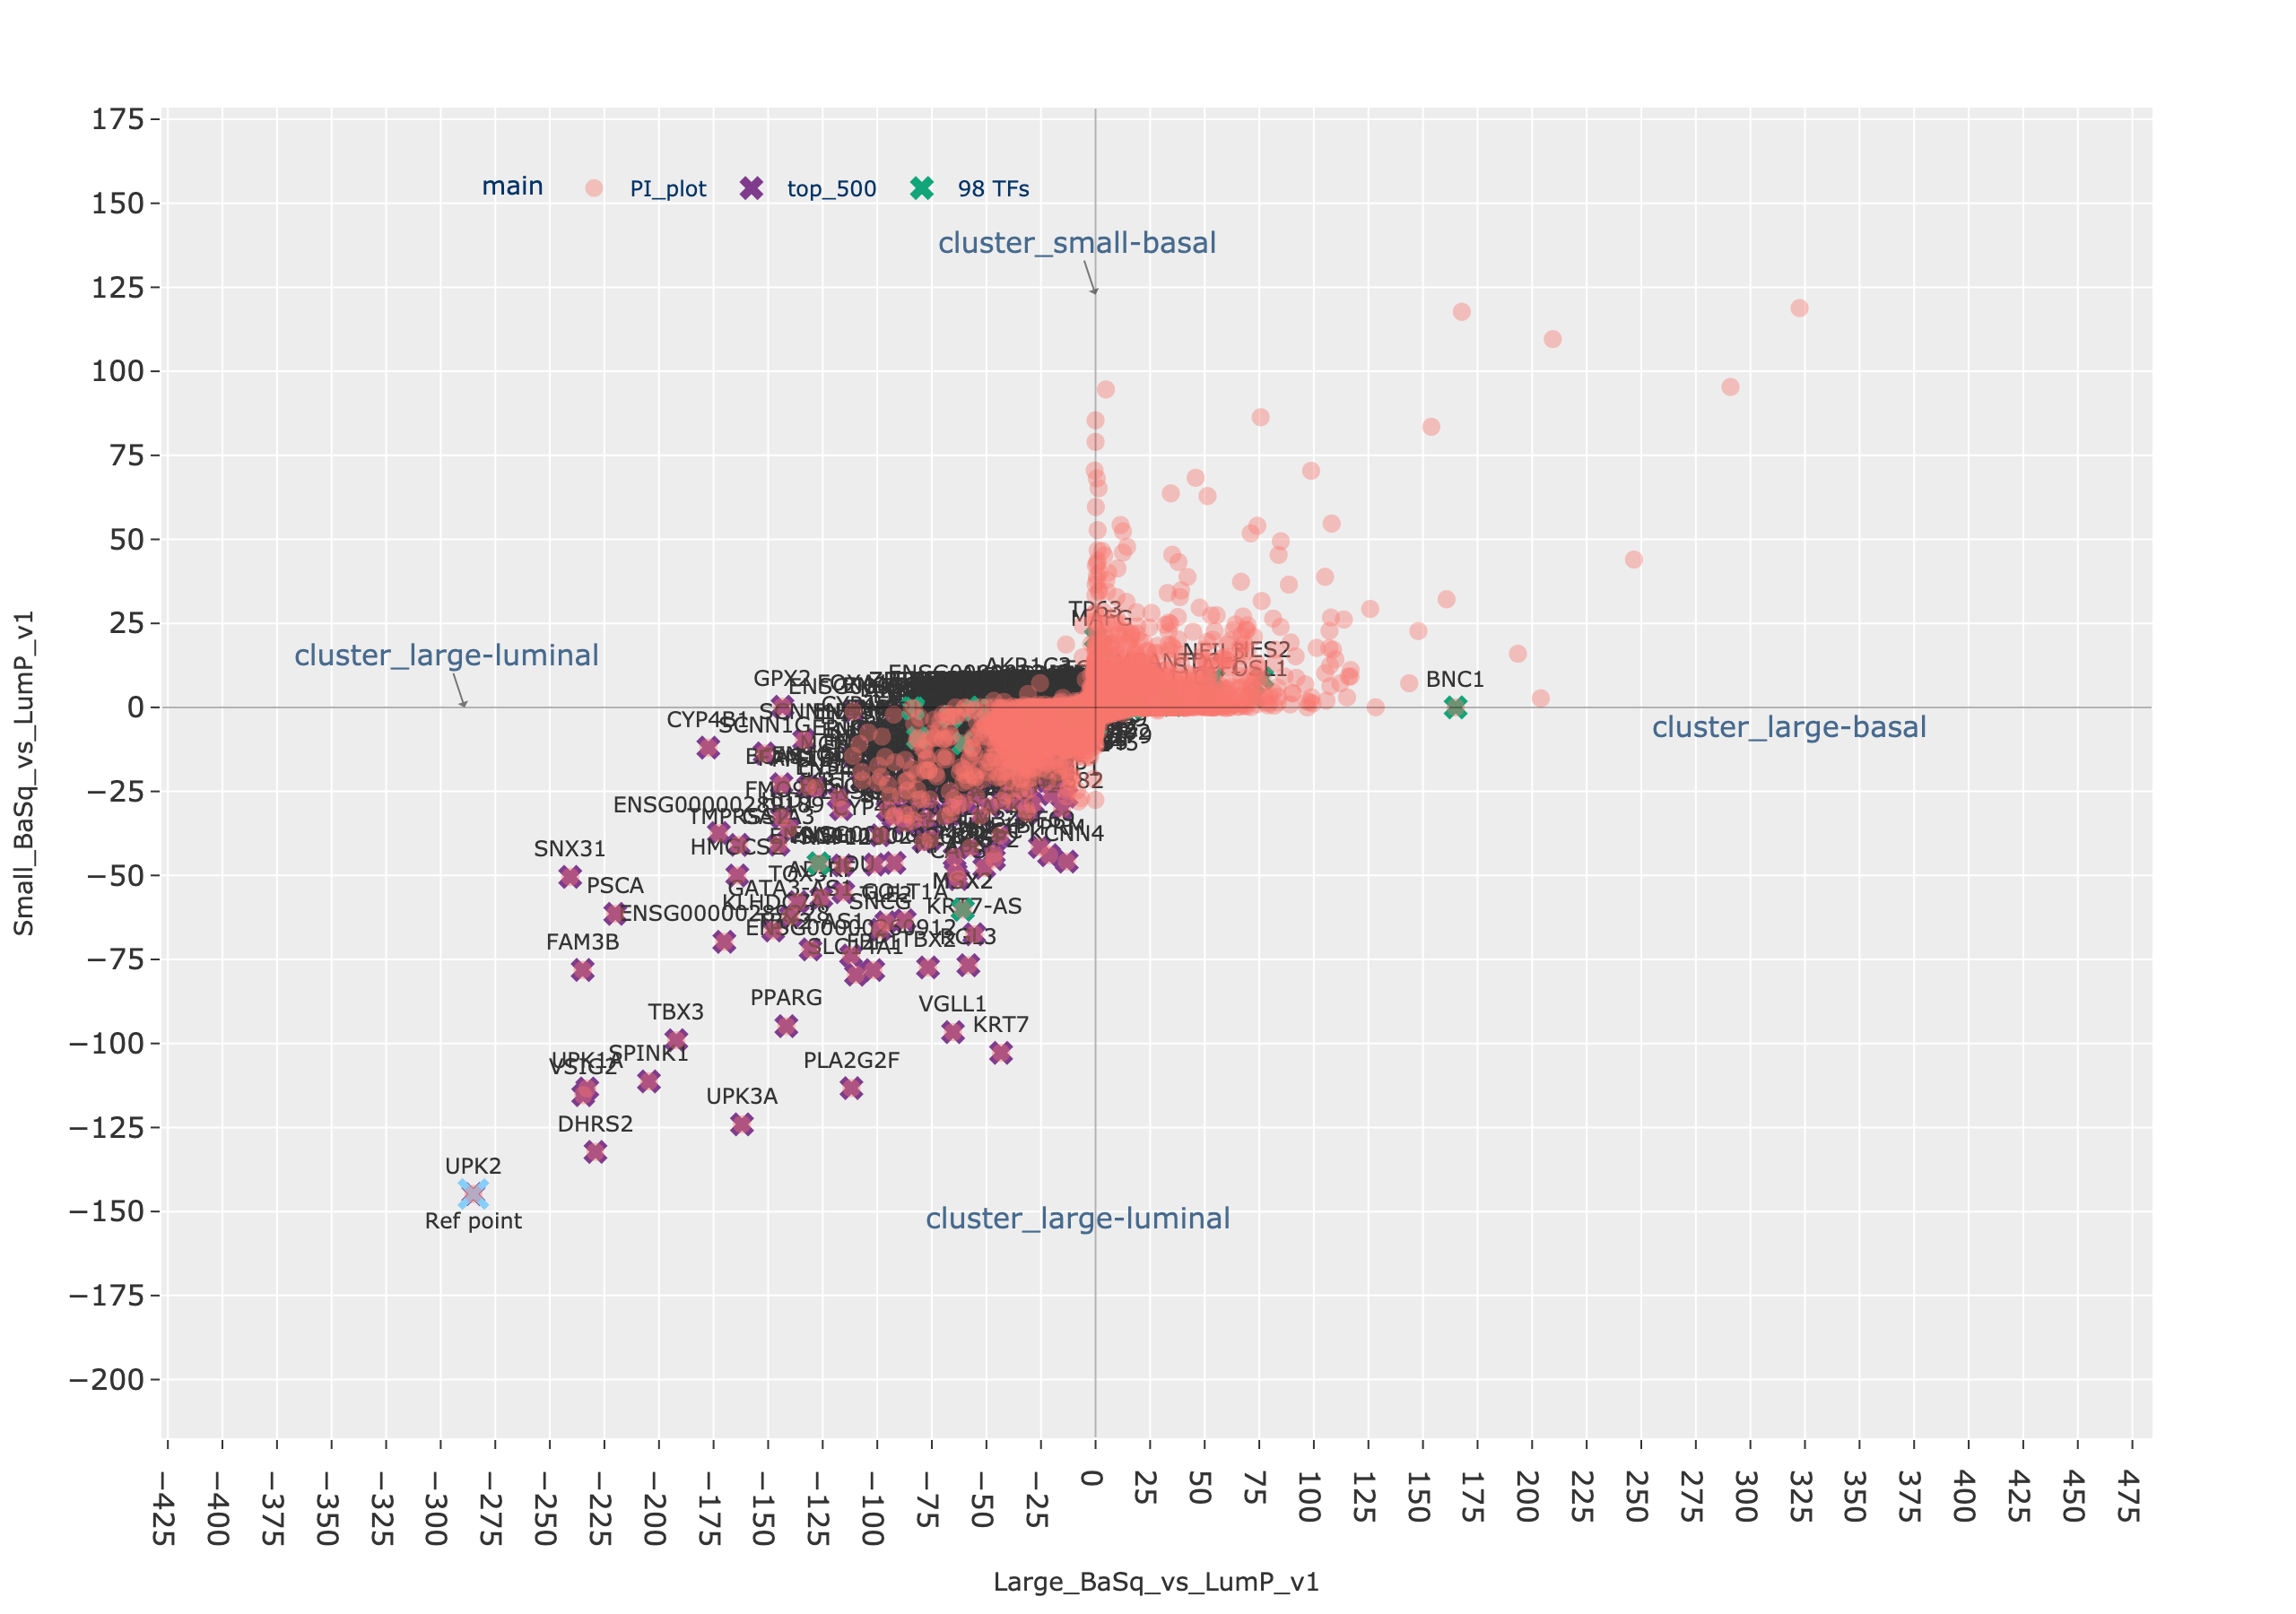
\includegraphics[width=\textwidth,keepaspectratio]{Sections/Network_I/Resources/selective_pruning/pi_gsea/pi_largeLuminal.png}
        \caption{Large luminal}
    \end{subfigure}\hspace{\fill} % maximize horizontal separation

    \caption{Pi plots for large basal and luminal explored in \cref{s:N_I:bio_sel_prun} -}
    \label{fig:ap:pi_large_basal}
\end{figure}

\begin{figure}[!h]
    \captionsetup[subfigure]{justification=Centering}
    \begin{subfigure}[!t]{0.9\linewidth}
        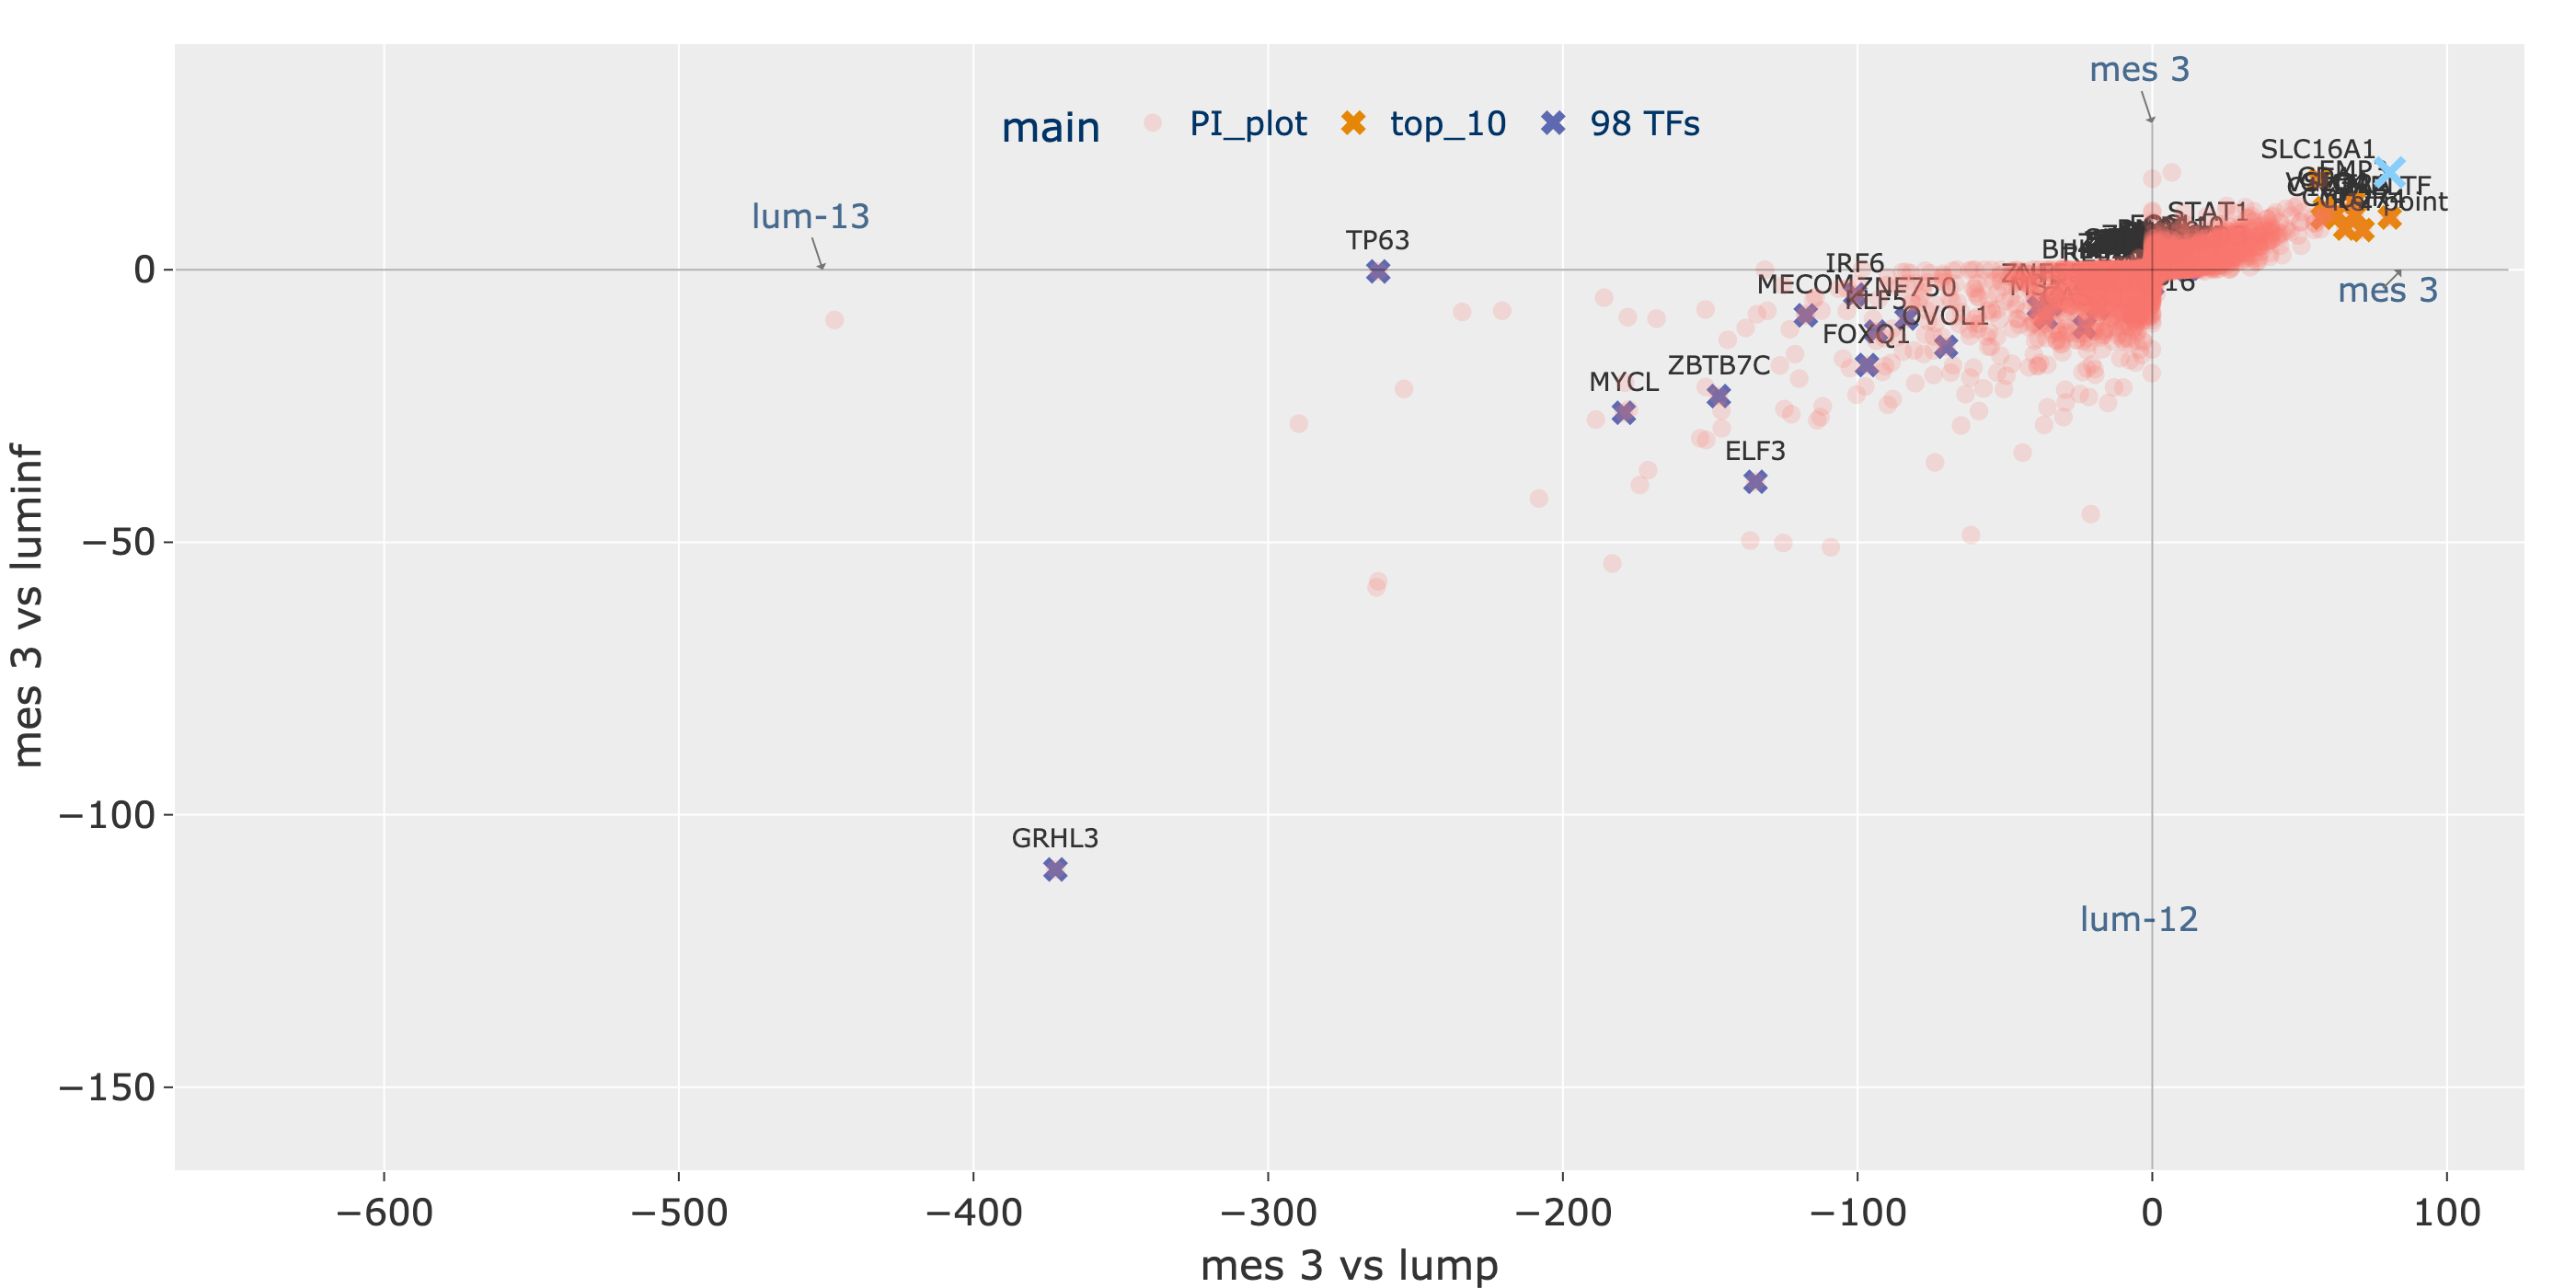
\includegraphics[width=\textwidth,keepaspectratio]{Sections/Network_I/Resources/selective_pruning/pi_gsea/pi_mesLike.png}
        \caption{Large Basal}
    \end{subfigure}\hspace{\fill} % maximize horizontal separation
    \begin{subfigure}[!t]{0.9\textwidth}
        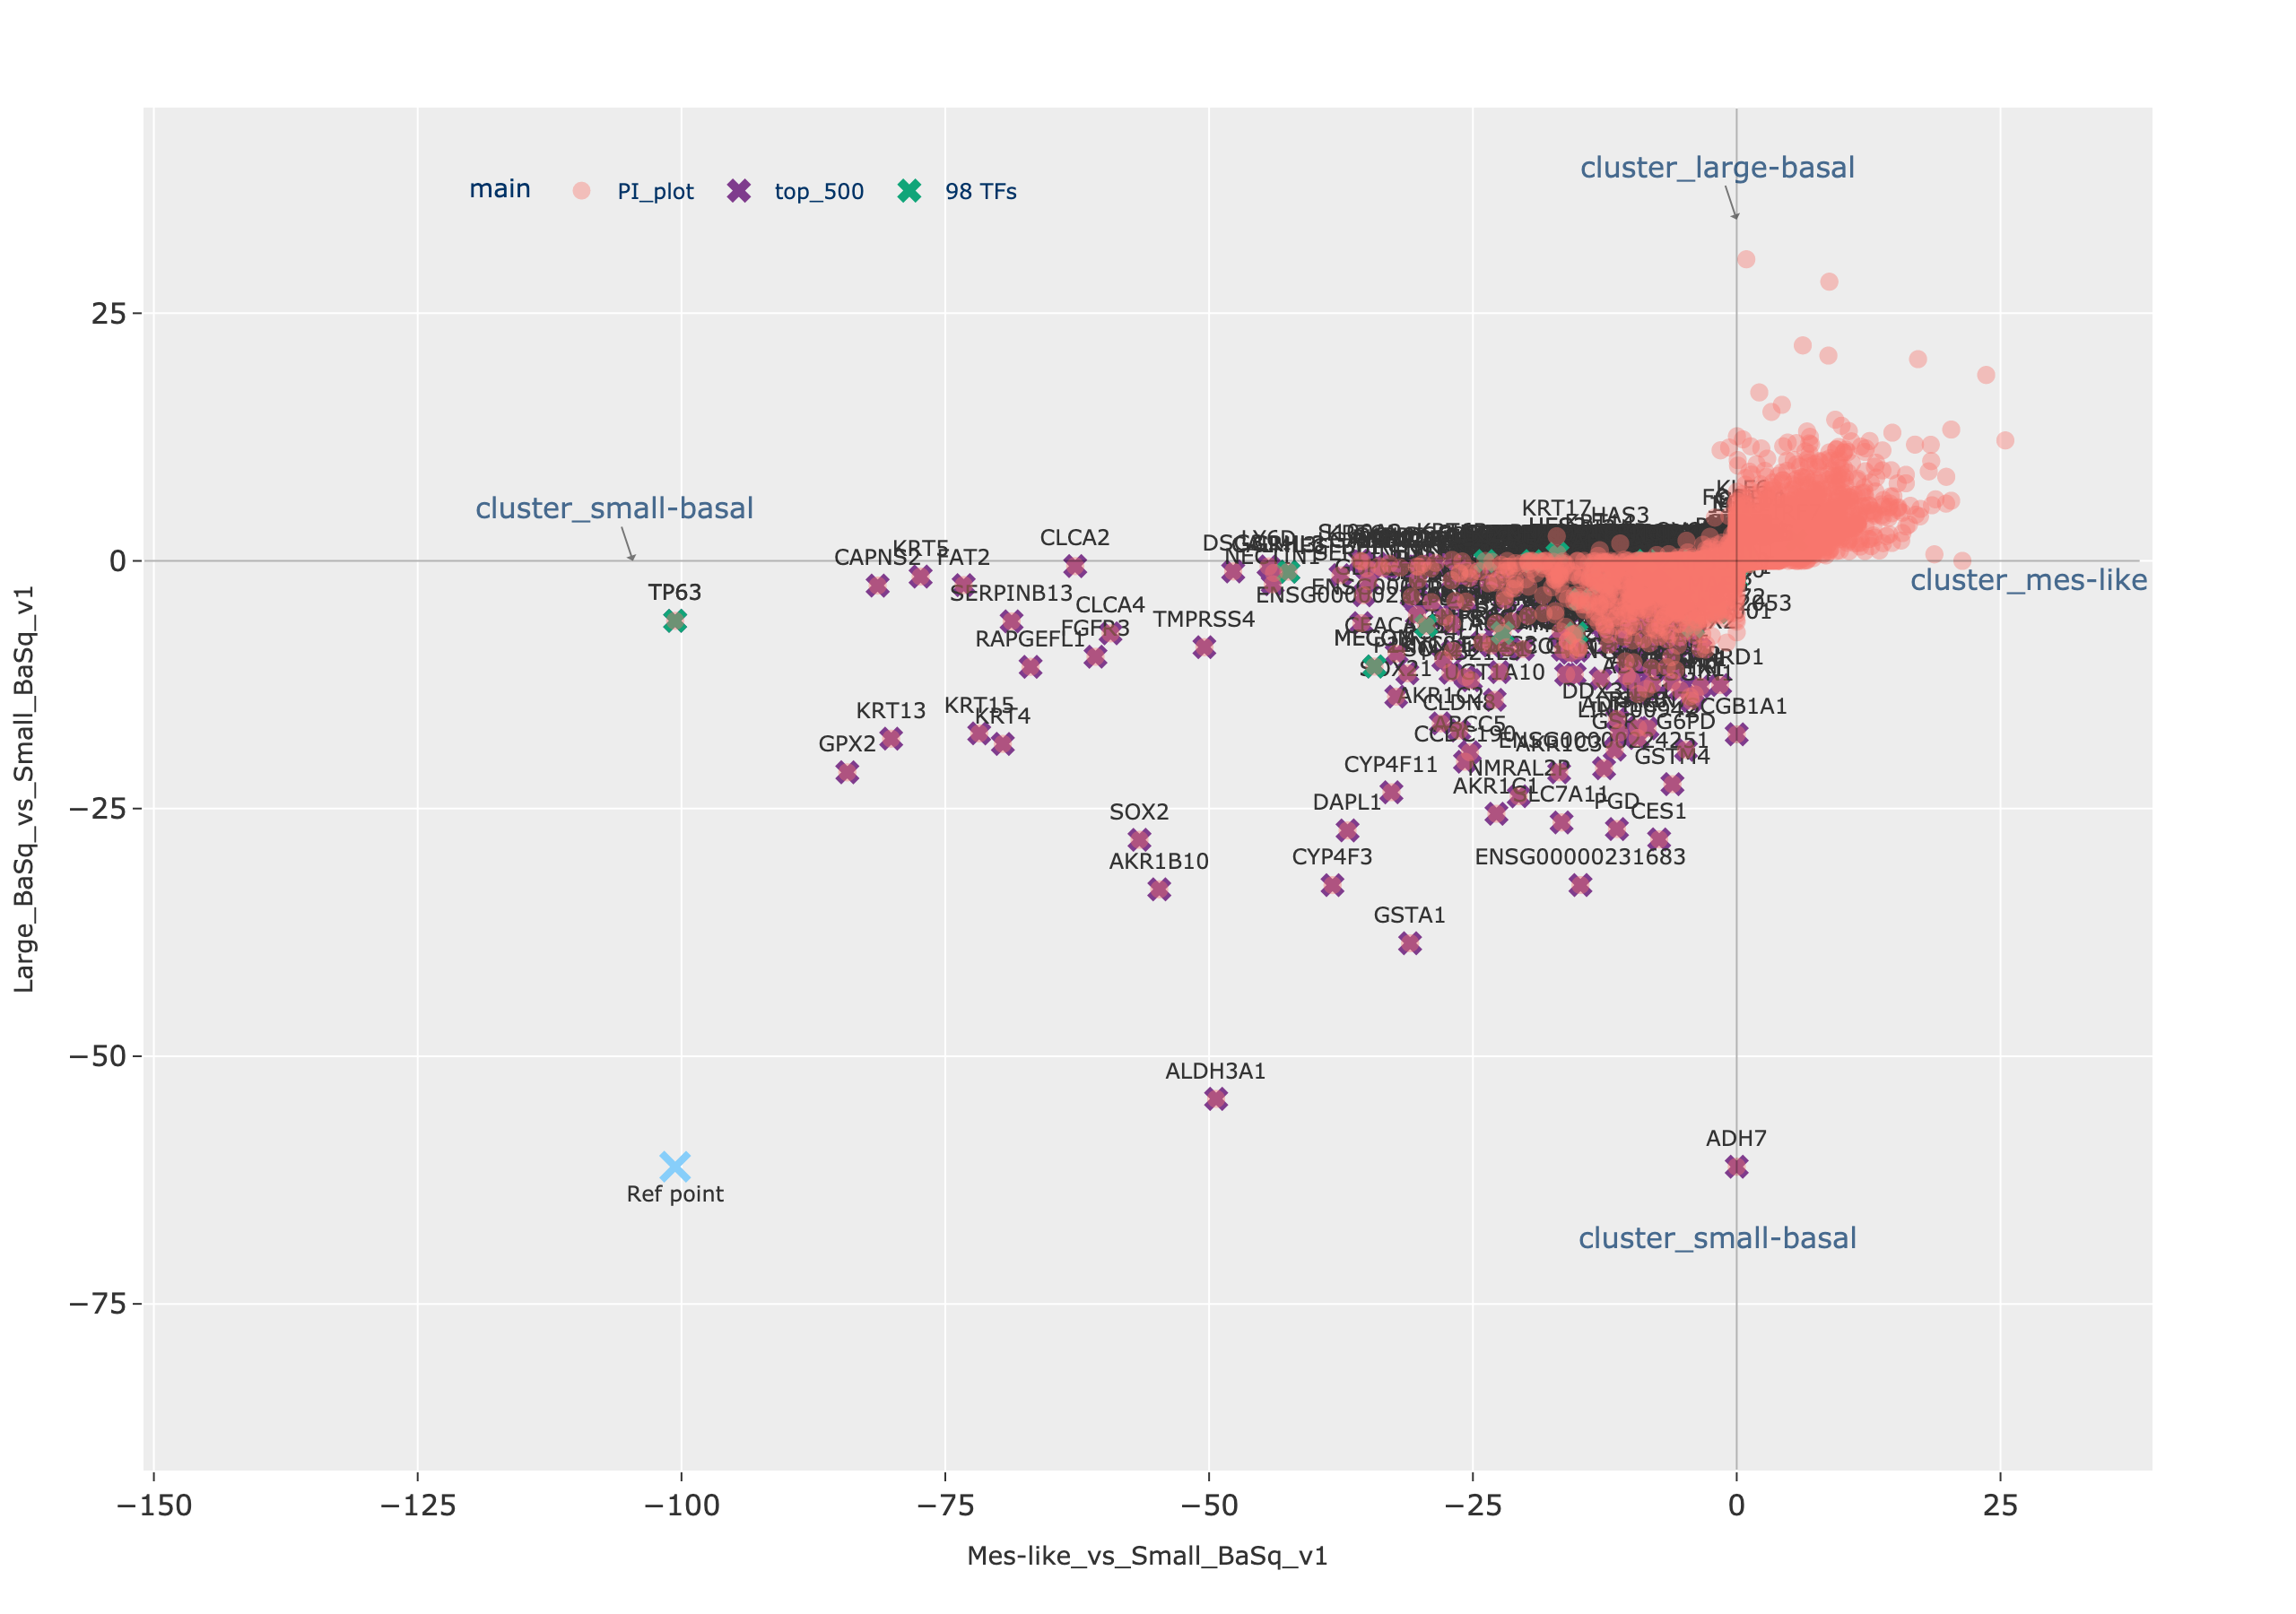
\includegraphics[width=\textwidth,keepaspectratio]{Sections/Network_I/Resources/selective_pruning/pi_gsea/pi_smallBasal.png}
        \caption{Large luminal}
    \end{subfigure}\hspace{\fill} % maximize horizontal separation

    \caption{Pi plots for mes-like and lumInf from \cref{s:N_I:bio_sel_prun}}
    \label{fig:ap:pi_lumInf_mesLike}
\end{figure}


% GSEA - hallmarks
\subsubsection{GSEA output - Hallmarks} \label{s:ap:hallmarks}

\begin{table}[H]
  \centering
  \scriptsize
  \begin{tabularx}{\textwidth}{>{\hsize=1.5\hsize}X|>{\hsize=0.4\hsize}X|>{\hsize=0.4\hsize}X|>{\hsize=0.6\hsize}X|>{\hsize=0.4\hsize}X|>{\hsize=0.4\hsize}X}
    \toprule
    \textbf{Term} & \textbf{NES} & \textbf{FDR q-val} & \textbf{\# lead} & \textbf{\# matched} & \textbf{ratio} \\
    \midrule
    \multicolumn{6}{c}{\textbf{smallBasal}} \\
    \midrule
    MYC TARGETS V1 & 1.909 & 0 & 149 & 40 & 0.268 \\
    \midrule
    MITOTIC SPINDLE & 1.887 & 0 & 138 & 61 & 0.442 \\
    \midrule
    TGF BETA SIGNALING & 1.863 & 0 & 28 & 15 & 0.536 \\
    \midrule
    \multicolumn{6}{c}{\textbf{largeBasal}} \\
    \midrule
    KRAS SIGNALING UP & 2.384 & 0 & 132 & 104 & 0.788 \\
    \midrule
    \multicolumn{6}{c}{\textbf{lumInf}} \\
    \midrule
    CHOLESTEROL HOMEOSTASIS & 1.892 & 0 & 33 & 20 & 0.606 \\
    \midrule
    APOPTOSIS & 1.733 & 0 & 61 & 37 & 0.607 \\
    \midrule
    \multicolumn{6}{c}{\textbf{largeLuminal}} \\
    \midrule
    DNA REPAIR & 1.617 & 0.004 & 77 & 12 & 0.156 \\
    \midrule
    PEROXISOME & 1.608 & 0.003 & 57 & 22 & 0.386 \\
    \midrule
    FATTY ACID METABOLISM & 1.552 & 0.004 & 71 & 38 & 0.535 \\
    \midrule
    PROTEIN SECRETION & 1.549 & 0.003 & 42 & 11 & 0.262 \\
    \midrule
    BILE ACID METABOLISM & 1.46 & 0.008 & 59 & 19 & 0.322 \\
    \bottomrule
  \end{tabularx}
  \caption{NES, FDR q-val, and lead gene statistics for different subtypes and terms in bladder cancer biology.}
  \label{ap:tab:gsea_hallmark}
\end{table}

% GSEA - oncoSig
\subsubsection{GSEA output - OncoSig} \label{s:ap:sel_prun_oncosig}

% Table for hallmarks
\begin{table}[H]
  \centering
  \scriptsize
  \begin{tabularx}{\textwidth}{>{\hsize=1.5\hsize}X|>{\hsize=0.4\hsize}X|>{\hsize=0.4\hsize}X|>{\hsize=0.6\hsize}X|>{\hsize=0.4\hsize}X|>{\hsize=0.4\hsize}X}
    \toprule
    \textbf{Term} & \textbf{NES} & \textbf{FDR q-val} & \textbf{\# lead genes} & \textbf{\# matchedl} & \textbf{ratio matched} \\
    \midrule
    \multicolumn{6}{c}{\textbf{smallBasal}} \\
    \midrule
    SINGH KRAS DEPENDENCY SIGNATURE & 2.121 & 0 & 17 & 10 & 0.588 \\
    \midrule
    TBK1.DF DN & 2.105 & 0 & 206 & 132 & 0.641 \\
    \midrule
    EIF4E DN & 2.084 & 0 & 53 & 44 & 0.83 \\
    \midrule
    PGF UP.V1 UP & 2.002 & 0 & 111 & 67 & 0.604 \\
    \midrule
    ERBB2 UP.V1 DN & 1.877 & 0 & 110 & 67 & 0.609 \\
    \midrule
    GCNP SHH UP LATE.V1 UP & 1.863 & 0 & 120 & 52 & 0.433 \\
    \midrule
    P53 DN.V1 UP & 1.862 & 0 & 68 & 65 & 0.956 \\
    \midrule
    RB P130 DN.V1 DN & 1.862 & 0 & 82 & 52 & 0.634 \\
    \midrule
    \multicolumn{6}{c}{\textbf{largeBasal}} \\
    \midrule
    CSR LATE UP.V1 UP & 2.382 & 0 & 115 & 86 & 0.748 \\
    \midrule
    TBK1.DF UP & 2.332 & 0 & 173 & 135 & 0.78 \\
    \midrule
    CSR EARLY UP.V1 UP & 2.326 & 0 & 110 & 74 & 0.673 \\
    \midrule
    \multicolumn{6}{c}{\textbf{mesLike}} \\
    \midrule
    CORDENONSI YAP CONSERVED SIGNATURE & 2.49 & 0 & 48 & 39 & 0.812 \\
    \midrule
    LEF1 UP.V1 UP & 2.423 & 0 & 125 & 110 & 0.88 \\
    \midrule
    RB P107 DN.V1 UP & 2.316 & 0 & 84 & 71 & 0.845 \\
    \midrule
    LTE2 UP.V1 DN & 2.265 & 0 & 118 & 86 & 0.729 \\
    \midrule
    \multicolumn{6}{c}{\textbf{lumInf}} \\
    \midrule
    BCAT.100 UP.V1 UP & 2.067 & 0 & 24 & 22 & 0.917 \\
    \midrule
    CSR LATE UP.V1 DN & 1.964 & 0 & 70 & 49 & 0.7 \\
    \midrule
    AKT UP.V1 DN & 1.889 & 0 & 90 & 66 & 0.733 \\
    \midrule
    ESC J1 UP LATE.V1 UP & 1.828 & 0 & 81 & 67 & 0.827 \\
    \midrule
    \multicolumn{6}{c}{\textbf{largeLuminal}} \\
    CSR EARLY UP.V1 DN & 1.679 & 0.002 & 73 & 32 & 0.438 \\
    \midrule
    MYC UP.V1 DN & 1.613 & 0.002 & 77 & 38 & 0.494 \\
    \bottomrule
  \end{tabularx}
   \caption{NES, FDR q-val, and lead gene statistics for different subtypes and terms in bladder cancer biology from the OncoSig database.}
  \label{ap:tab:gsea_oncosig}
\end{table}


\end{appendices}
